\documentclass[letterpaper, onecolumn,10pt,draftclsnofoot]{IEEEtran}
\usepackage{lipsum}
\usepackage[final]{pdfpages}
\usepackage{graphicx}
\usepackage{amssymb}
\usepackage{amsmath}
\usepackage{amsthm}

\usepackage{alltt}
\usepackage{caption}
\usepackage{float}
\usepackage{color}
\usepackage{url}
\usepackage{listings}
\lstset{ 
   language=C++,                % choose the language of the code
   basicstyle=\small,        % the size of the fonts that are used for the code
   keywordstyle=\color{blue},
   stringstyle=\color{red},
   commentstyle=\color{green},
   numbers=left,                   % where to put the line-numbers
   numberstyle=\footnotesize,      % the size of the fonts that are used for the line-numbers
   stepnumber=1,                   % the step between two line-numbers. If it is 1 each line will be numbered
   numbersep=5pt,                  % how far the line-numbers are from the code
   backgroundcolor=\color{white},  % choose the background color. You must add \usepackage{color}
   showspaces=false,               % show spaces adding particular underscores
   showstringspaces=false,         % underline spaces within strings
   showtabs=false,                 % show tabs within strings adding particular underscores
   frame=single,           % adds a frame around the code
   tabsize=2,          % sets default tabsize to 2 spaces
   captionpos=b,           % sets the caption-position to bottom
   breaklines=true,        % sets automatic line breaking
   breakatwhitespace=false,    % sets if automatic breaks should only happen at whitespace
   escapeinside={\%*}{*)}          % if you want to add a comment within your code
   }
   \usepackage{balance}
   \usepackage[TABBOTCAP, tight]{subfigure}
   \usepackage{enumitem}
   \usepackage{pstricks, pst-node}

   \usepackage{geometry}
   \usepackage{longtable,hyperref}
   \geometry{textheight=8.5in, textwidth=6in, margin=0.75in}
 
   \renewcommand*\rmdefault{cmr}

   \newcommand{\cred}[1]{{\color{red}#1}}
   \newcommand{\cblue}[1]{{\color{blue}#1}}
   \newcommand{\itab}[1]{\hspace{4em}\rlap{#1}}


   \title{Final Report}
   \author{Hailey Palmiter, Scott Griffy, and Ryan Kitchen}
   \date{\today}

   %% The following metadata will show up in the PDF properties
   \hypersetup{
      colorlinks = true,
      urlcolor = black,
      pdfauthor = {Palmiter, Griffy, Kitchen},
      pdftitle = {HawkEye Final Report},
      pdfsubject = {CS463},
      pdfpagemode = UseNone
   }
   \begin{document}
   \begin{titlepage}
	\centering
       	\vfill
       
	\begin{figure}[H] 
	\centering
	
\includegraphics[width=0.6\textwidth,natwidth=610,natheight=642]{images/HawkEye_Logo.png}  
	\end{figure}

	\vfill
	{\bfseries\Large
	 Image Processing Vision System for Manned and Unmanned Aircraft\\
	 \vskip.5cm
         CS 463 - Senior Capstone Final Report\\
         \vskip.5cm
         June 10th, 2016\\
         \vskip1cm
         Group 4 - HawkEye Crew\\ 
         \vskip.5cm
         Hailey Palmiter\\
         \vskip.5cm
         Scott Griffy\\
         \vskip.5cm
         Ryan Kitchen\\
        }
    
      \vfill
      \vskip2cm
      \begin{abstract} 
	  This document is a final report constructed using the IEEEtran style guidelines. The report provides an introduction to our senior project, a project description, and a personal overview from each member of the team about what they learned over the course of the project. The report includes our original requirements document, design document, and technological review with an added discussion about each document. This discussion describes how the project has changed over the course of the year in comparison to how it was perceived during the planning process. Also included is our weekly blog posts that were been generated over the course of the year to keep our TA and our sponsors up to date with our progress. We also included our final poster that was used at the Engineering Expo. Appendix 1 covers essential code listings and appendix 2 displays the hardware we used and a few output images from our vision system. 

      \end{abstract}
      \vfill
   \end{titlepage}
   
   \onecolumn
   \tableofcontents
   \newpage
   \bigskip
\IEEEraisesectionheading{\section{Introduction}\label{sec:introduction}}
	Rockwell Collins, our project sponsor, designs video vision systems for pilots to use during flight. Pilots often use these enhanced image systems to help them see better in rough weather conditions, and to generally assist during different flight operations such as landing. An example of this functionality could be overlaying a pilot's view with graphics to help the pilot locate a landing strip in a storm or automatically turning a night-vision camera off when it is not needed in order to save power. The hardware used for this system must limit the power consumption it pulls from the aircraft, and also must be lightweight as weight is a very expensive resource on aircraft. Even an extra five pounds added to the plane during a year can add up to thousands of dollars in fuel costs. In order to provide pilots with enhanced image processing while maintaining low power consumption and low weight, Rockwell Collins develops software on Field Programmable Gate Arrays (FPGAs). While it meets the power and weight requirements, this piece of hardware makes the code very complex and very costly to develop. New vision enhancements can take weeks or months to develop on the FPGAs. The FPGAs are currently Rockwell Collins only option that meets the requirements needed to create practical systems that pilots can use effectively.\\
\par
Our goal is to provide a proof of concept for an alternative to Rockwell Collins' FPGAs. It must meet the performance metrics, provide faster implementation time, and reduce the cost of production. Specifically, we are designing a proof of concept using single board computers (SBCs). Single board computers differ from FPGAs because they have a standardized execution environment, which allows simpler code to be executed on it, reducing the development time. Single board computers also use low cost hardware and don't consume much power. If we can prove that the video quality produced by the SBCs is adequate for pilots to use, they will meet all the requirements needed to develop a practical vision system. In the air, FPGAs often take feeds from multiple cameras and run a lot of processing algorithms on those images. In order to be effective, the SBCs should also be able to handle this operation. Our project aims to test and measure the capabilities of a single board computer by delivering a multiple-stream video display that has been processed to a high degree. We believe the best candidate for this is to use NVIDIA's single board computer: the Jetson TX1. Our goal is to fully test the Jetson TX1's ability to provide enhanced imaging. This proof of concept will result in measurements that will help Rockwell Collins determine the practicality of using single board computers for their vision systems.\\
\par
   %About clients roles and who they were, team members and our roles%
Our clients are Carlo Tiana and Weston Lahr through Rockwell Collins.
The members of the HawkEyed Crew are: Scott Griffy, Hailey Palmiter, and Ryan Kitchen.
Ryan Kitchen worked on the technical side of the project. Scott helped with some of the technical side and wrote documentation. Hailey edited and wrote documentation and managed the project.
We communicated with the clients to define requirements and secure hardware necessary for the project. We also got a lot of the hardware from our instructor, Kevin McGrath.


\newpage
\section{Original Requirements Document}
	\subsection{Introduction}
\subsubsection{Purpose}
Rockwell Collins currently develops their vision systems on Field Programmable Gate Arrays, making the time from design to product very long.  Rockwell Collins is considering using Single Board Computers as a way to speed up this cycle.
Our goal is to provide a proof of concept for a vision system on a Single Board Computer for Rockwell Collins. This proof of concept should help Rockwell Collins measure the practicality of Single Board Computers for vision systems.\\

\subsubsection{Scope}
Development will be limited to the Jetson TK1 or Jetson TX1. Evaluation of hardware platforms other than the TK1 and TX1 will be a stretch goal. In which case, these boards will serve as the base unit for comparison. Software shall interface to a minimum of 2 cameras, receive video, and display it on a monitor while logging metrics. Metrics will be frames per second and operations per second.\\

\subsubsection{Definitions}
\begin{description}[leftmargin=2cm,labelindent=2cm]
	\item [SBC] Single board computer
	\item [RC] Rockwell Collins
	\item [FPS] Frames per second
	\item [FPGA] Field-programmable gate array
	\item [USB] Universal serial bus
	\item [PoC] Proof of concept
	\item [SVS] Simple vision system\\
\end{description}

\subsubsection{References}
Carlo Tiana, Airborne Vision Systems Expert at Rockwell Collins
Weston Lahr, Senior Software Engineer at Rockwell Collins,
Jetson TK1 Embedded Hardware, NVIDIA\\

\subsubsection{Assumptions and Constraints}
We're assuming that either Jetson model can handle some sort of camera vision system. From initial investigations it appears that the Jetson TX1 is a likely candidate to support our project goals.

\subsection{Overall Description}
This section will give a bird's eye view of the project, outlining the major features and their purpose.\\
\subsubsection{Product Perspective}
  \paragraph{System Interfaces}
  Linux, Jetson Distro
  \paragraph{User Interfaces}
  While using our deliverable, the user should be able to view output image from the Jetson.
  \paragraph{Software Interfaces}
  Our deliverable should be a demonstrate of the Jetson's video output, charts that display capability performance, information about the complexity and amount of video processing operations. A stretch goal would include to have the same output of the software running on a second screen.
  \paragraph{Hardware Interfaces}
  We must choose an interface between our program and the chosen camera attached to the Jetson SBC. We must also interface with the relative camera processing systems on the Jetson.
  \paragraph{Communication Interfaces}
  We will communicate with at least two different camera streams, from two separate cameras attached to our SBC.\\
  
\subsubsection{Product Functions}
The delivered demonstration should accurately demonstrate the performance limitations of the Jetson TK1 or TX1. Should the timeframe allow, we are to continue investigating other SBCs and providing a similar overview of other researched SBCs.\\

\subsubsection{User Characteristics}
Our users will be RC developers, looking to implement a given filter for vision processing platforms.\\

\subsubsection{Constraints}
Our deliverable must run on either the Jetson TK1 or Jetson TX1, and should simply test the Jetson's capabilities. We will use 1080p cameras.\\

\subsubsection{Assumptions and Dependencies}
We are assuming that the Jetson can at least handle some level of video processing.We are also going to rely on libraries and the operating system provided by Nvidia for the Jetson.\\

\subsubsection{Stretch Goal Timeline}
Stretch goals defined throughout this document may be delayed until all other requirements are finished and are not required to be in the deliverable at any point.

\subsection{Specific Requirements}
This section will outline some of the more specific parts of the project along with exact requirements that the deliverable should meet.\\

\subsubsection{External Interfaces}
\begin{description}[leftmargin=2cm,labelindent=2cm]
	\item [Two 1080p Cameras] These will be used to transfer video data to the Jetson to be processed and displayed on a monitor.
	\item [Monitor] Any monitor able to adequately display the output of the chosen SBC for the purposes of evaluation. 
	\item [Jetson] Should be able to read and process video data and stream it out to a monitor.\\
\end{description}

\subsubsection{Functions}
The system shall take input from the cameras and perform as much video processing on it as possible before dipping under the 30 fps minimum.
If the system can't handle 30fps without any extra video processing, it should simply be displayed at the fastest fps possible.\\

\subsubsection{Performance Requirements}
The system should support at least 2 cameras with a stretch goal of 3 cameras.
The system should support video output on one monitor, and if possible the video should be displayed at 30fps.\\

\subsubsection{Design Constraints}
Since this is a proof of concept, the only real design constraint is that it should be able to correctly assess and demonstrate the hardware limitations of the Jetson SBC.\\

\subsubsection{Maintainability}
Maintainability, outside of our timeframe, is a low-priority requirement as we are only delivering a proof of concept for the capabilities of our SBC.\\

\subsubsection{Portability}
Our software should give some idea of how similar code would perform on other platforms, even though the PoC itself does not have to be portable. The same goes for the camera and monitor.In order to help our stretch goal of evaluating a second SBC, it would help if the code, cameras, and monitor were all collectively portable to the second platform.\\

\subsection{Stretch Goals}
Some stretch goals were listed throughout the requirements. One purpose of the stretch goals is to further increase the effectiveness of the proof of concept. These added goals further stress the limitations of the Jetson TK1 or TX1, to further expand the capabilities of these SBC. A few other stretch goals not mention above would be implementing the same system on a similar SBC, and comparing that with the Jetson TK1 or TX1, or implementing object tracking as a video processing operation to test performance of the SBCs.\\

\subsection{Gantt Chart}
\begin{figure}[H] 
\centering
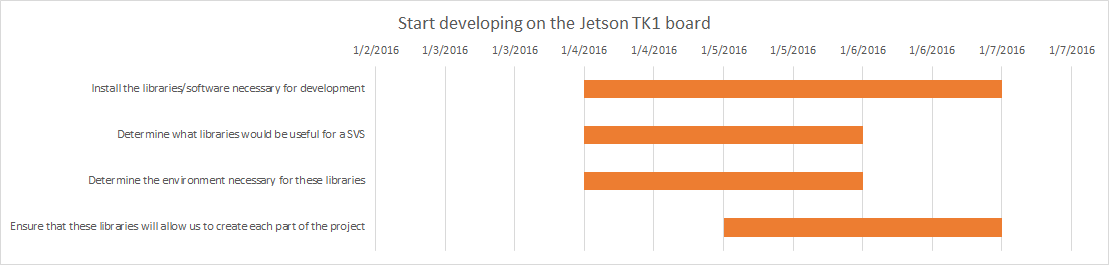
\includegraphics[width=1.0\textwidth,natwidth=1210,natheight=642]{gantt/original/starting.png}  
\end{figure}
\begin{figure}[H] 
\centering
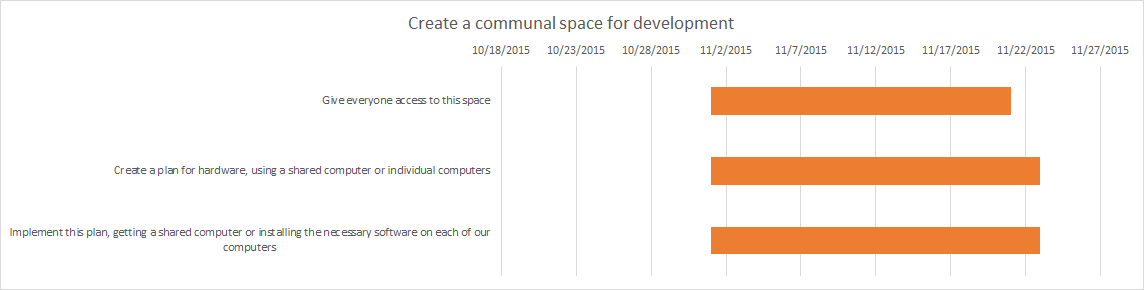
\includegraphics[width=1.0\textwidth,natwidth=1210,natheight=642]{gantt/original/communal.png}  
\end{figure}
\begin{figure}[H] 
\centering
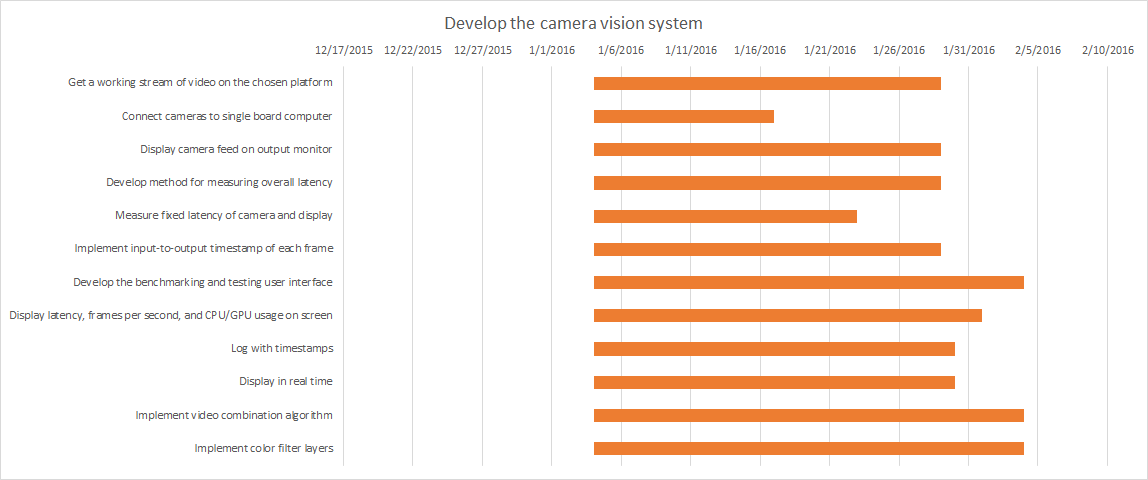
\includegraphics[width=1.0\textwidth,natwidth=1210,natheight=642]{gantt/original/develop.png}  
\end{figure}
\begin{figure}[H] 
\centering
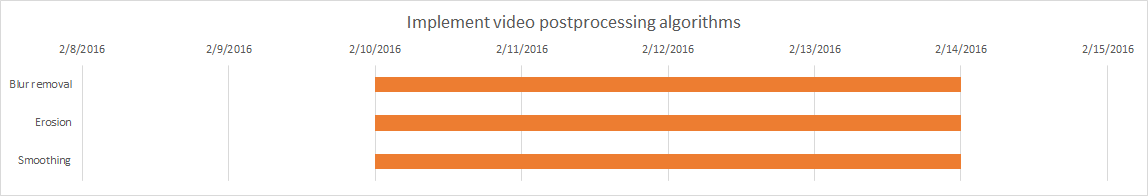
\includegraphics[width=1.0\textwidth,natwidth=1210,natheight=642]{gantt/original/algos.png}  
\end{figure}
\begin{figure}[H] 
\centering
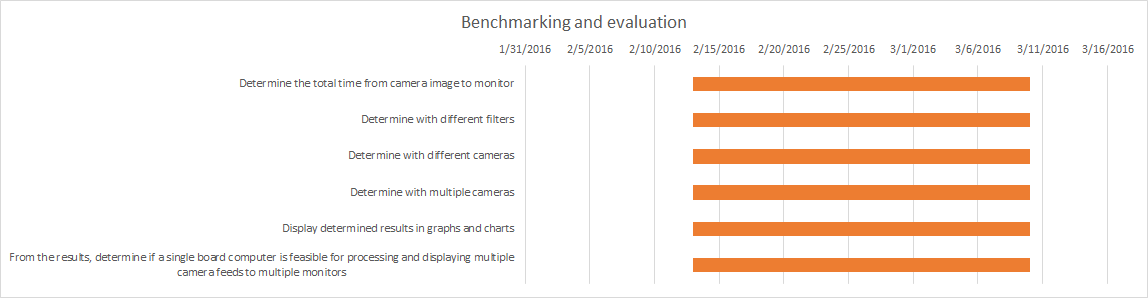
\includegraphics[width=1.0\textwidth,natwidth=1210,natheight=642]{gantt/original/eval.png}  
\end{figure}
\begin{figure}[H] 
\centering
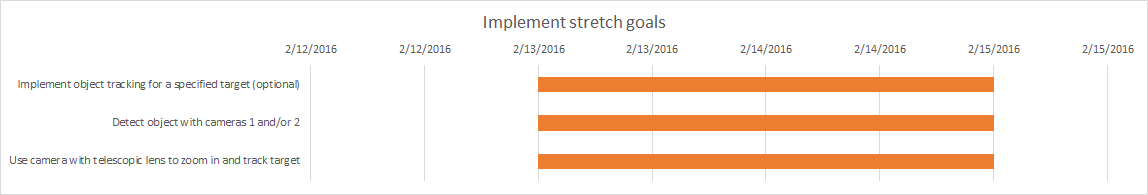
\includegraphics[width=1.0\textwidth,natwidth=1210,natheight=642]{gantt/original/stretch_goals.png}  
\end{figure}



\newpage
\section{Requirements Document Changes}
	Before real development began, we had reread our requirements document and noticed that some changes and additions needed to be made. The revision was needed in order to refine our project with the discovery of problems/improvements we had found. It was a needed process as we wanted to have full clarity on what needed to be accomplished with this project, and be able to display those requirements with our sponsor. The changes were reviewed with our sponsor and agreed upon before any final changes were made.
\par
Only a few minor things were changed, but they had a big impact on how we define our deliverable according to their standard. Our client was very happy to see the revisions we had made and all final revisions were made in conjunction with our document. The table below shows the minor changes we had made.\\

\begin{center}
	\begin{tabular} { | c | c | c | p{5cm} | }
	\hline
	\multicolumn{ 4 } { | c | } {Requirements Document Changes} \\
	\hline
	1 & Two Working Cameras &  Added Requirement &  In our original document we had not specified more than one camera, but our sponsor specifically wanted to make that a requirement as the system must be able to handle more than one camera. Therefore it was added into our requirements document.\\ \hline
	2 & Use of Either Jetson TK1 or TX1  & Redefined Requirement  &  Before the revision, the requirements document was specifying the use of only the Jetson TK1. After much research on our end we had decided that either Jetson's TK1 or TX1 would be adequate for development, and actually plan to rely more heavily on the Jetson TX1. This change allows us to have more flexibility between the two Jetson SBC's, which provides protection if we cannot get one to work properly or to the meet the requirements needed.\\ 
	\hline
	\end{tabular}
\end{center}
	\subsection{Final Gantt Chart}
	\begin{figure}[H] 
\centering
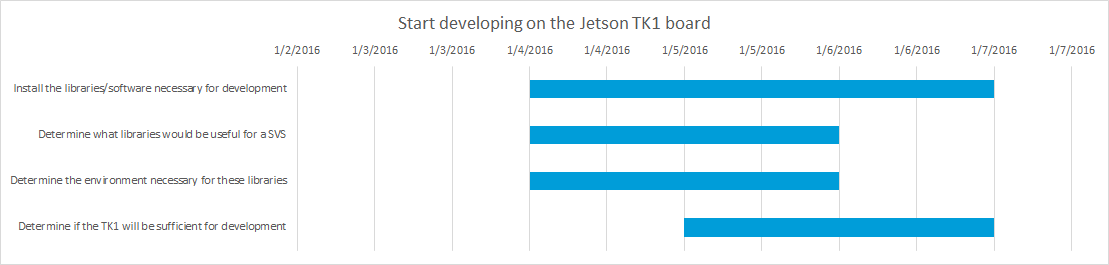
\includegraphics[width=1.0\textwidth,natwidth=1210,natheight=642]{gantt/final/starting.png}  
\end{figure}
\begin{figure}[H] 
\centering
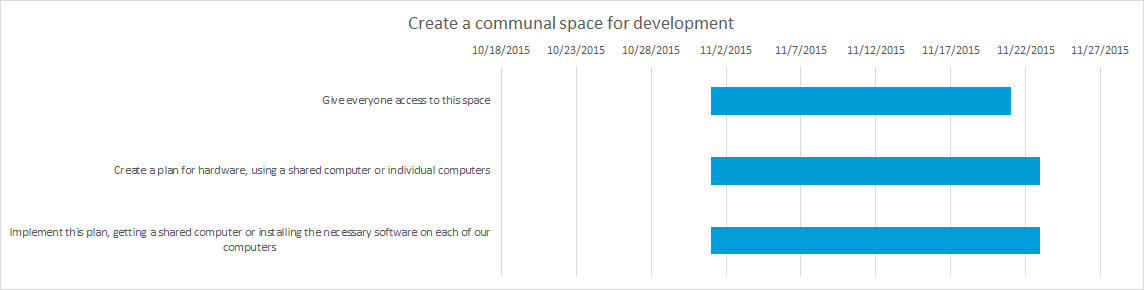
\includegraphics[width=1.0\textwidth,natwidth=1210,natheight=642]{gantt/final/communal.png}  
\end{figure}
\begin{figure}[H] 
\centering
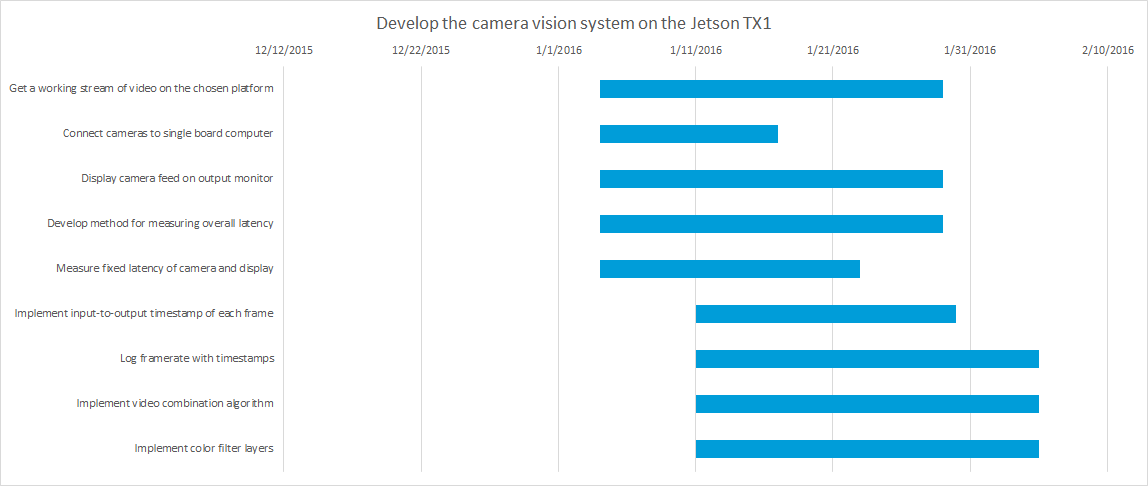
\includegraphics[width=1.0\textwidth,natwidth=1210,natheight=642]{gantt/final/develop.png}  
\end{figure}
\begin{figure}[H] 
\centering
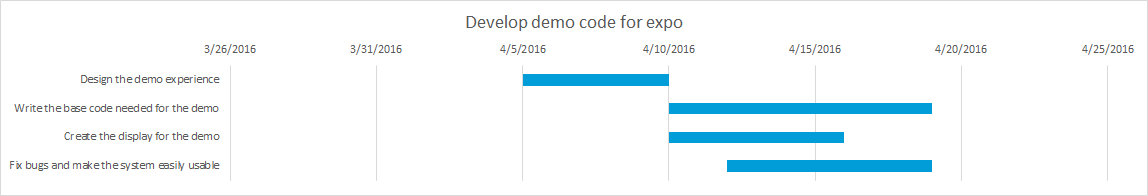
\includegraphics[width=1.0\textwidth,natwidth=1210,natheight=642]{gantt/final/algos.png}  
\end{figure}
\begin{figure}[H] 
\centering
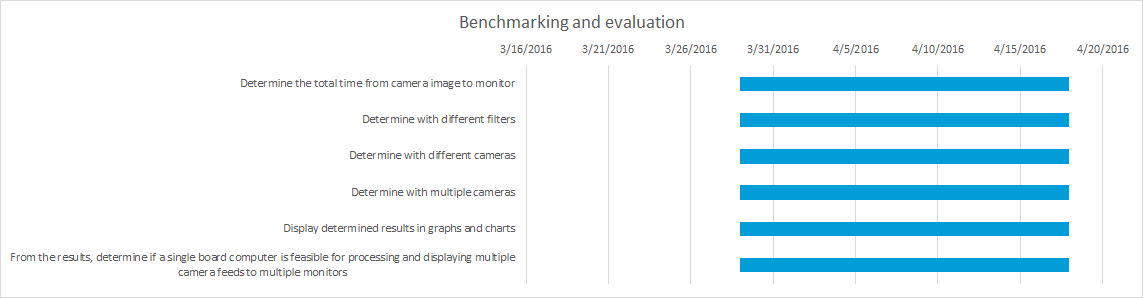
\includegraphics[width=1.0\textwidth,natwidth=1210,natheight=642]{gantt/final/eval.png}  
\end{figure}
\begin{figure}[H] 
\centering
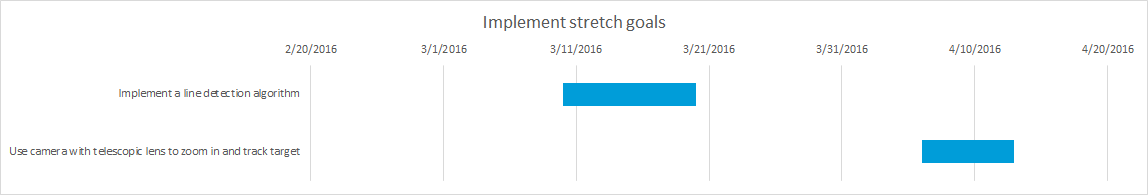
\includegraphics[width=1.0\textwidth,natwidth=1210,natheight=642]{gantt/final/stretch.png}  
\end{figure}


\newpage
\section{Design Document}
	\subsection{Introduction}
\subsubsection{Scope}
This software will implement a framework to develop, test, and benchmark video processing
algorithms. The users will be able to test different combinations of algorithms using one or multiple
camera inputs and produce output to one or multiple display windows. This software will be used by
HawkEye Crew to determine if the Nvidia Jetson TK1 or other off the shelf single board computers have
high enough performance to replace FPGA-based video processing systems currently used by Rockwell
Collins.\\
\subsubsection{Purpose}
This software description document will provide HawkEye Crew with a road map to complete
development of the software and fulfill the requirements in our Software Requirements Specification.
This document explains how the system is going to work, who is going to use it, and how it is meant to
be used.\\
\subsubsection{Intended Audience}
The intended audience of this design document is the developers who will design the system \(us\)
and the sponsors of this project at Rockwell Collins.\\
\subsubsection{References}
IEEE. IEEE Std 1016-2009 IEEE Standard for Information Technology \- System Design \- Software
Design Descriptions. IEEE Computer Society, 2009

\subsection{Definitions}
\begin{description}[leftmargin=2cm,labelindent=2cm]
	\item [SBC] Single board computer
	\item [RC] Rockwell Collins
	\item [FPS] Frames per second
	\item [FPGA] Field-programmable gate array
	\item [USB] Universal serial bus
	\item [PoC] Proof of concept
	\item [UML] Unified Modeling Language
	\item [DFD] Data Flow Diagram: Shows how data moves between different components in the system
	\item [ER Diagram] Entity Relationship Diagram: Shows how different data structures within the software are connected to each other
	\item [SDD] Software Design Description
	\item [SRS] Software Requirements Specification
	\item [SVS] Simple Vision System
	\item [YUV] A color space typically used as part of a color image pipeline
	\item [JSON] JavaScript Object Notation
	\item [Modular Video Processing System] The HawkEye Video Processing System's internal video processing algorithm management and execution system.\\
\end{description}

\subsection{Conceptual Model for Software Description}
\subsubsection{Software Design in Context}
For the HawkEye Video Processing System, we will be using a functional design method. Our
system is designed to be modular and have standardized interfaces, so we will be able to develop new
features and drop them in without modifying existing code. The reasoning for using a functional design
rather than object oriented is because our software is focused on processing individual video frames in
real time. Each algorithm instance will run once and has no state, only input and output data. For that
reason functional programming is the best choice for this design.\\

\subsubsection{Software Design Descriptions within the Life Cycle}
This document details how we are going to the implement software to meet our requirements.
During the course of development, our requirements and our SRS may be updated. This document
includes support for both our current requirements and provides room to add additional requirements.
It also adds additional operational requirements and functionality beyond those specified in the
requirements document. This document will also provide a reference for the creation of our testing plan.

\subsection{Design Architecture}
\subsubsection{Stakeholder Concerns and Requirements}
Our client Rockwell Collins would like to know if single board computers are a viable option to
implement simple vision systems on. They've enlisted us, the HawkEyeCrew, to implement a proof of
concept to measure the effectiveness of single board computers in this context.
\par
We, the HawkEye Crew, will be using this software to test various implementations of video
processing algorithms. In order for our system to be a valid proof of concept, our system will need to
meet certain performance benchmarks and functional requirements described by our SRS. Our design
concerns will be meeting these requirements.\\
\subsubsection{Description of Architectural Design}
Our system is designed to be a framework and testbed for the implementation of video
processing algorithms. This design handles the hardware input interface, video output to the monitor,
data flow between different algorithms, parallel operation of multiple operations, and benchmarking of
individual components and overall aggregate timing.
\par
In order to provide maximum flexibility and testing capabilities, the video processing algorithms and
input/output devices are built as separate, interchangeable modules. These different modules are
organized by the user in a configuration file, which determines both how the modules connect to each
other and how the log file is formatted. This enables us to track the performance of individual
algorithms and maximize our CPU and GPU usage while maintaining the performance requirements for
this project.\\
\subsubsection{Validation of Design}
The core requirements of our system that this design either implements or implements the
capability of testing are as follows:\\
\begin{enumerate}[leftmargin=2cm,labelindent=2cm]
\item System must be capable of processing multiple video streams
\item System must enable thorough testing of the Jeston's video processing capabilities
\item Frame rate must be at least 30FPS
\item End to end latency must be less than 100ms\\
\end{enumerate}

These requirements are met by the following architectural features:\\
\begin{enumerate}[leftmargin=2cm,labelindent=2cm]
\item The modular video processing system enables multiple input and output devices.
\item The modular video processing system will enable us to maximize the usage of CPU and GPU
processing power, which will show the maximum performance of the Jetson.
\item This software design includes built in speed benchmarking, so we will be able to track FPS.
\item This benchmarking system also produces latency details, so we will be able to determine if this
system is capable of meeting the latency requirements Rockwell Collins is looking for.\\
\end{enumerate}

\subsubsection{Overview of Viewpoints and Design Languages}
These viewpoints have been chosen to provide a complete description of the design and show
how the design is compliant with the SRS. Each one provides details crucial to understanding how the
design works and is a reference for implementation.\\

\begin{enumerate}[leftmargin=2cm,labelindent=2cm]
\item \textbf{Context viewpoint:}
This viewpoint shows the different potential users of the software and how they would
interact with our system.\\
Design Languages: Use Case Diagram
\item \textbf{Structure viewpoint:}
This viewpoint shows how the streaming video flows through the system, and identifies the
internal and external data connection points in the system. This viewpoint also shows the
components of the system which enable connection of cameras via USB as per the SRS.\\
Design Languages: Data Flow Diagram
\item \textbf{Interaction viewpoint:}
This viewpoint shows the order of operations on processing a video frame, as well as how
the timing is integrated to meet the performance benchmarking requirement.\\
Design Languages: UML Sequence Diagram
\item \textbf{Information viewpoint:}
This viewpoint details how the modular video processing system determines the order of
operations for the various elements and algorithms it can create. It shows how the system
meets the requirement for modularity and the capability to use multiple input and output
devices.\\
Design Languages: Entity Relationship Diagram
\item \textbf{State Dynamics Viewpoint:}
While the algorithm implementations in our design are stateless, the system itself is not.
This viewpoint shows the transitions between different states and provides a road map for
different states which will need to be individually tested.\\
Design Languages: UML State Transition Diagram
\end{enumerate}

\subsection{Design Viewpoints}
\subsubsection{Context Viewpoint}

	\paragraph{Users and Design Concerns}
	The design features in this document are chosen to create value for several different
kinds of users and stakeholders. These users interact with the software in different ways.\\
	\begin{enumerate}[leftmargin=2cm,labelindent=2cm]
    	\item \textbf{Pilot:}
	Our intended user will be a pilot of a manned or unmanned aerial vehicle. This software
	is designed to provide increased and extensible functionality for onboard camera
	systems. Because our product is a proof of concept, there won't be a real pilot, but the
	pilot has been included as a user because the application of this design is to create
	better equipment for pilot use. This pilot will be 'using' our product and needs the
	video stream to meet the requirements outlined in the SRS.
	\item \textbf{Distributor:}
	Rockwell Collins is the sponsor and primary stakeholder in this project. They will
	evaluate the product and decide where to use it. They will also decide the feasibility of
	using this design in production and whether continuing to use single board computers
	for real-time video processing is a good idea.
	\item \textbf{Implementer:}
	The implementer has to set up the simple vision system on their given hardware. Our
	proof of concept should give some notion as to how to do this and also the feasibility
	and easiness of it. The concepts demonstrated in this design document can be used on
	different hardware, not just the NVIDIA Jetson.
	\item \textbf{Algorithm Designer:}
	The algorithm designer interacts with our software in different ways than the end user
	and implementer. This user will create custom modules and link them together with our
	easy to use configuration system. This configuration should serve as a design for other
	systems.\\
	\end{enumerate}
	
	\paragraph{Use Case Diagram}
	
	\begin{minipage}{\linewidth}
		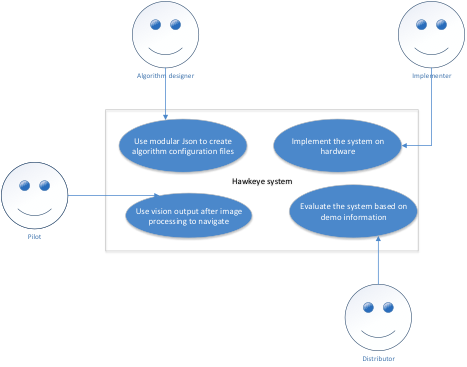
\includegraphics[keepaspectratio=true,scale=0.6]{images/UseCase_Diagram.png}
		%\begin{figure}[H] %\textwidth,natwidth=610,natheight=642
		%\centering
		%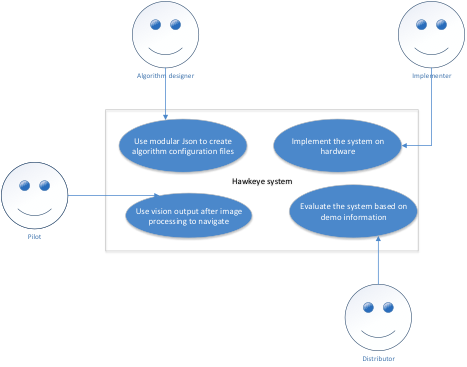
\includegraphics[width=0.6\textwidth,natwidth=610,natheight=642]{images/UseCase_Diagram.png} 
		%\caption{Use Case Diagram}\label{UseCase_Diagram.png} 
		%\end{figure}
		
	\end{minipage}
	
\subsubsection{Structure Viewpoint}
This section shows the high level organization of our software design.  
	\paragraph{Design Concerns}
	The primary design concern of this section is to show the interaction between critical components of our software design. This is valuable during implementation because it provides a reference for the required parts of the system, and also shows how the different pieces fit together.\\
	\paragraph{Design Elements}
	There are three key design elements in our software design. These elements are important because they are the basis for the entire modular video processing system.\\
	
	\begin{enumerate}[leftmargin=2cm,labelindent=2cm]
	\item \textbf{Video Buffer:}
	Shared data space provided by video4linux or created internally. Video data is in YUV format and access is provided through a void pointer to a 	contiguous block of memory.
	\item \textbf{Algorithm Module:} 
	Algorithm modules are single purpose elements that operate on one or more input buffers and provide output to one or more output buffers. They 	consist of a C function which performs the operations, and a module definition structure which provides the name and expected input and outputs 	of a module. 
	\item \textbf{Algorithm Controller:}
	This element is responsible for ordering and executing Algorithm Modules. It is the primary routine in this software design. It reads from a JSON 	configuration file, creates a module execution tree, and manages the execution of concurrently running modules.\\
	\end{enumerate}
	
	\paragraph{Structure Description}
	The HawkEye video processing software receives frames from the Video4Linux driver as a pointer to a buffer. The Algorithm Controller invokes each video processing algorithm in the order described by the configuration file, by passing them pointers to the buffers assigned to them. The video processing algorithms perform actions directly on the video buffer in order to avoid the performance hit from accessing additional memory. When the last video processing algorithm is complete, the buffer is flushed to the output device.\\
	
	\paragraph{Data Flow Diagram}
	\begin{figure}[H] 
		\centering
		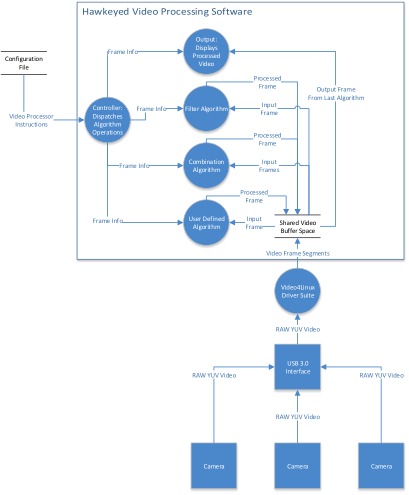
\includegraphics[width=0.6\textwidth,natwidth=610,natheight=642]{images/DataFlow_Diagram.png}  
		\end{figure}
	
\subsubsection{Interaction Viewpoint}
	\paragraph{Design Concerns}
	The main goal of this project is to determine how much video processing can be done on a SBC while maintaining a frame rate of 30 FPS and latency below 100ms. To this end, we as the user have two design concerns that need to be addressed.\\
	
	\begin{enumerate}[leftmargin=2cm,labelindent=2cm]
	\item \textbf{Latency measurement:}
	In order to keep overall latency under 100ms while maximizing the amount of processing being done, we need to know how long each algorithm 	takes to process a single frame, and also how long it takes from input to output.

	\item \textbf{FPS Monitoring:}
	Our software must process video in real time. For the purposes of this project, that has been specified as 30 FPS by our SRS. This is separate 	from the latency requirement because our system may actually be operating on multiple frames simultaneously, so the frames per second may not 	necessarily dictate the total latency.\\
	\end{enumerate}
	
	\paragraph{Design Elements}
	This viewpoint contains several design elements that depict major components of our software design.\\
	
	\begin{enumerate}[leftmargin=2cm,labelindent=2cm]
	\item \textbf{Camera Buffer:}
	Initially, camera buffer will store the data immediately loaded by the camera and will then be repurposed to hold the modified image later. This 		modified image will come from the custom algorithm code.

	\item \textbf{Custom Algorithm:}
	The custom algorithm is loaded into the system when it starts up through the JSON configuration files and dynamically linked libraries. This 		portion of the system will perform operations on the camera buffer and log the time at start and time at completion. It will then write back to the 		camera buffer, the modified image.

	\item \textbf{Log:}
	The log is a feed that will keep track of the frame rate and information about what processes are running. This should be viewable separately from 	the display.

	\item \textbf{Display:}
	The last thing that should happen when we are rendering frames is the stream to the display. This will show the final, completely processed 		image. Our client has contacted us and told us that the display should only show the video stream, not other metrics like frames per second or 		operations per frame.

	\item \textbf{Video4Linux Camera Driver:}
	This is our direct access point to the video stream from the USB camera. It enables us to receive video frames from any cameras supported by 	the Linux operating system.\\
	\end{enumerate}
	
	\paragraph{UML Sequence Diagram}
	\begin{figure}[H] 
		\centering
		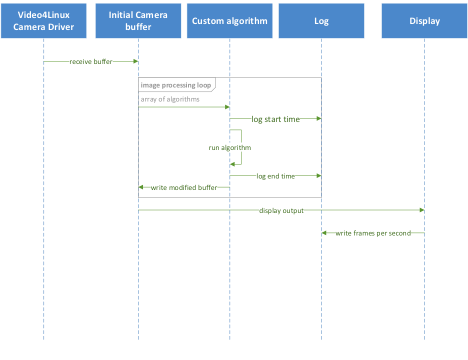
\includegraphics[width=0.6\textwidth,natwidth=610,natheight=642]{images/UML_Diagram.png}  
		\end{figure}
	
\subsubsection{Information Viewpoint}
	\paragraph{Design Concerns}
	
	\begin{enumerate}[leftmargin=2cm,labelindent=2cm]
	\item \textbf{Configuration:}
	This viewpoint addresses how the user will configure our software. It shows how the modules are connected to each other and the information that 	needs to be provided for the software to create its internal structure.

	\item \textbf{Internal Data Structure:}
	In order to implement the modular image processing system, our design needs an internal data structure in order to determine the execution path 	through the various modules.\\
	\end{enumerate}
	
	\paragraph{Design Elements}
	There are two design elements in this viewpoint:\\
	\begin{enumerate}[leftmargin=2cm,labelindent=2cm]

	\item \textbf{Module Instances:}
	Module instances are C structures that describe either input device modules, output device modules, or algorithm execution modules. They 		consist of a name, type, and the names of the connected input and output modules.
	\item \textbf{JSON Configuration File:}
	In order to create the internal data structure for our application, the user must write a configuration file in JSON format. The elements in this 		configuration file are detailed in an example below (Example JSON Configuration File).\\
	\end{enumerate}
	
	\paragraph{Description and Rationale}
	The HawkEye video processing software needs to be able to handle various configurations of multiple camera inputs and produce multiple outputs, as well as performing multiple video processing algorithms. In order to do this, it needs to know what operations to perform in what order, and where to put the data. To do this, our software uses a tree-like data structure that connects the camera inputs, algorithm modules, and outputs. An input module definition specifies what modules a camera sends data to. Each of those modules then has its own output specification, which can either go to another algorithm module or an output module. \\
	
	\paragraph{Sample Entity Relationship Diagram}
	\begin{figure}[!h] 
		\centering
		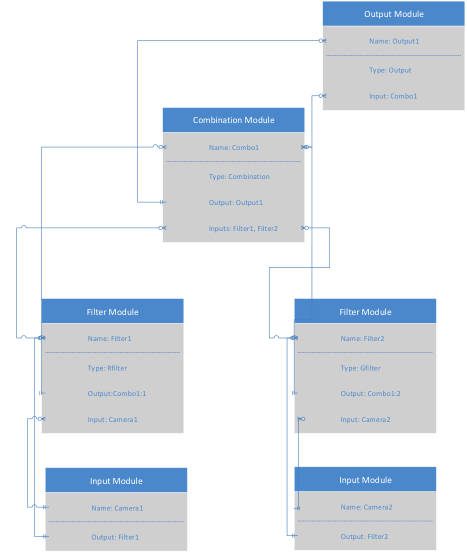
\includegraphics[width=0.6\textwidth,natwidth=610,natheight=642]{images/ER_Diagram.png}  
		\end{figure}
	
	\paragraph{Example JSON Configuration File}
	The corresponding JSON configuration file for the above ER diagram. \\
	
	 \begin{lstlisting}
	 {
   	 	"Output1":{
        			"type":"output",
        			"input":"Combo1"
    		},
    		"Combo1":{
        			"type":"Combination",
        			"inputs":"Filter1,Filter2",
        			"output":"Output1"
    		},
   		 "Filter1":{
        			"type":"Rfilter",
        			"input":"Camera1",
        			"output":"Combo1:1"
    		},
    		"Filter2":{
        			"type":"Gfilter",
        			"input":"Camera2",
        			"output":"Combo1:2"
    		},
    		"Camera1":{
       		 	"type":"Input",
        			"device":"/dev/video0",
        			"output":"Filter1"
    		},
    		"Camera2":{
        			"type":"Input",
        			"device":"/dev/video1",
        			"output":"Filter2"
   		 },
    		(not used in this example but also an option)
    		"Tracker":{
        			"type":"Module",
        			"filename":"tracker.so"
   	 	}
	}
	 \end{lstlisting}
	
	The one rule for the JSON files is that each entity must be declared before its inputs; this top down approach enables the JSON parsing algorithm to generate the module tree in a single pass. The one exception to this rule is cyclical algorithms that operate on their own output, either directly or indirectly. Support for such algorithms may be implemented, but this is not part of the current project scope. 
	
\subsubsection{State Dynamics Viewpoint}
	\paragraph{Design Concerns}
	Our program will be in multiple states while it is streaming and processing data from the camera to the display. In order to keep track of the states, we will have two state diagrams, one for the camera and a second for the software for processing.\\
	
	\paragraph{Design Elements}
	
	\begin{enumerate}[leftmargin=2cm,labelindent=2cm]
	\item \textbf{Camera:}
	For the purposes of this viewpoint, Camera shall refer to the combination of the physical camera hardware and the system level driver that exists 	outside of the HawkEye video processing application.

	\item \textbf{Software:}
	Refers to the HawkEye video processing application.\\
	\end{enumerate}
	
	\paragraph{Overview}
	The camera must be initialized before we can capture frames from it. After initialization the camera is ready for image capture. During image capture, the camera will write to a buffer on the host system. Once a frame has been written to the buffer, the software can begin image processing using the first algorithm in its configuration. When the algorithm is completed, the software will check if there is another algorithm to be performed. These two states of image processing and checking for more algorithms will loop until all algorithms have been completed. We will then write the finished image buffer to the screen. After that, we will check if the program needs to continue running or if it has received a shutdown command. To shut down we will finalize the camera, deactivate it, and stay in that state. \\
	\paragraph{States}
	
	\begin{enumerate}[leftmargin=2cm,labelindent=2cm]
	\item \textbf{Camera Initializing:}
	This is the starting state. Before we can capture frames from the camera, we must first initialize it. In this state we will also set up and synchronize the memory shared by the camera and our software.

	\item \textbf{Camera Initialized:}
	After we have initialized the camera it will be ready for capture. The software will have to start the camera's frame capture.

	\item \textbf{Camera Capturing:}
	The camera will take a moment to capture the data.

	\item \textbf{Camera Writing:} 
	The camera will have to write the data to memory. 

	\item \textbf{Image Reading:}
	Importing data from the camera's output into the software. This step should be simultaneous with camera writing as we are using the same 		memory. 

	\item \textbf{Image Processing:} 
	The image data in the buffer will be processed in place by the modular video processing system.

	\item \textbf{Process completed:}
	Once the algorithm is done operating, it will notify the controller that it has finished.

	\item \textbf{Write to Display:}
	The software will write the finalized image buffer to the display, displaying the video.

	\item \textbf{Camera Finalizing:}
	During this state, the camera is sending any remaining data and shutting down.

	\item \textbf{Camera Shut Down:}
	The camera is turned off. \\
	\end{enumerate}
	
	\paragraph{State Transition Diagram}
	Because the two state machines interact often, we have combined them in the same graphic. The following is our UML state machine:\\
	\begin{figure}[H] 
		\centering
		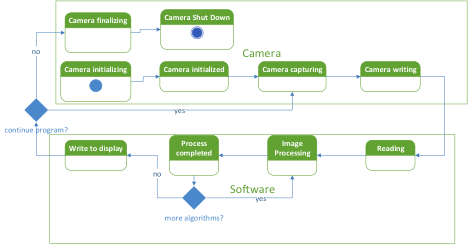
\includegraphics[width=0.6\textwidth,natwidth=610,natheight=642]{images/StateTransition_Diagram.png}  
		\end{figure}


\section{Design Document Changes}
	\subsection{Overall Description Changes}
We ended up having a physical copy of the performance of the system at expo instead of working it into our software. This was because we were advised that using the software to measure it's own performance would lead to problems, leading us to measure the performance of the system using a high speed camera which can't be done automatically.
\subsection{Specific Requirements}
One of the goals of the original design document was to create requirements that were reasonably achievable. Because of this mindset, the requirements in the document did not change very much.
\subsection{Information Viewpoint}
We had originally intended to create a modular json system, but scrapped it later on because it wasn't very valuable and created unecessary complexity.
   

\newpage
\section{Technology Review}
	\subsection{Camera Interface (Hardware Level)}
There are three different camera interfaces available on the Jetson development board. Each one offers a different set of benefits and challenges.\\
	\subsubsection{USB 3.0}
	USB 3.0 is a high-speed plug and play interface that offers a theoretical 384 MB/s data throughput. One USB 3.0 port is available on the Jetson, but 		additional ports can be added using the mini PCI Express expansion slot.\\

	Benefits:
	\begin{itemize}[leftmargin=2cm,labelindent=2cm]
		\item Availability of USB 3.0 cameras
		\item Plug and play, with no camera configuration
	\end{itemize}
	
	Drawbacks:
	\begin{itemize}[leftmargin=2cm,labelindent=2cm]
		\item Jetson onboard USB 3.0 does not meet the USB 3.0 specification for bandwidth
		\item Some cameras do not have USB 3.0 drivers for ARM
		\item USB 3.0 only supports one camera per port due to bandwidth limits
		\item Increased cost due to board expansion\\
	\end{itemize}
	
	\subsubsection{Gigabit Ethernet}
	The Jetson has one-gigabit Ethernet port available. Gigabit ports can handle 125 MB/s, however like USB 3.0 there are expansion cards available that add two additional ports.\\
	
	Benefits:
	\begin{itemize}[leftmargin=2cm,labelindent=2cm]
		\item All gigabit cameras use a standardized interface and require no driver
		\item More high quality cameras available than the USB 3.0 offers
		\item Simple configuration with video4linux
	\end{itemize}
	
	Drawbacks:
	\begin{itemize}[leftmargin=2cm,labelindent=2cm]
		\item Most cameras require external power supplies
		\item Gigabit cameras typically cost more than the USB 3.0 alternatives\\
	\end{itemize}
	
	\subsubsection{MIPI Camera Interface}
	The Tegra K1 processor on the Jetson has a direct camera interface, which is designed for onboard, low power camera modules. There are two MIPI interfaces, one 4 channel and one 1 channel interface, but any additional interfaces are unavailable.\\
		
	Benefits:
	\begin{itemize}[leftmargin=2cm,labelindent=2cm]
		\item High speed, built in interface
		\item Low power consumption
		\item Lower latency because the video processing can be done before buffering
	\end{itemize}
	
	Drawbacks:
	\begin{itemize}[leftmargin=2cm,labelindent=2cm]
		\item Very limited number of cameras supported
		\item Specific to the Tegra K1, making it not portable
		\item Increased hardware complexity
		\item Increased software complexity due to lack of standardized drivers\\
	\end{itemize}
	
	\subsubsection{Decision}
	We decided to use the USB 3.0 cameras because of the availability of low-cost high-quality cameras. Also, Rockwell Collins has several USB cameras they would like us to use. For our customer, it will be best to base the system around the USB 3.0 option. This may require adding a USB expansion card, but the other advantages of using USB 3.0 make it the first choice for camera connection.
	
\subsection{Video Subsystem (Software Level)}
We will have a framework for streaming the video from different components (camera, image processing unit, display).\\
	
	\subsubsection{OpenCV}
	We could use OpenCV to stream the video and setup processing of the video stream. This seems like the easiest approach, but would constrict us to the functions given by OpenCV, which might be enough for a proof-of-concept.\\
		
	Benefits:
	\begin{itemize}[leftmargin=2cm,labelindent=2cm]
		\item Able to write scripts using python
		\item Can use OpenCL to take advantage of the GPU
	\end{itemize}
	
	Drawbacks:
	\begin{itemize}[leftmargin=2cm,labelindent=2cm]
		\item Hides functionality
		\item Questionable performance\\
	\end{itemize}
	
	\subsubsection{Direct Memory Handling}
	We could handle the video stream ourselves on top of v4l provided by the Jetson, but would require some low-level knowledge of the Jetson's hardware. It would allow for more control over the video stream and give better performance.\\
	
	Benefits:
	\begin{itemize}[leftmargin=2cm,labelindent=2cm]
		\item Fast performance
		\item Full control of operations
	\end{itemize}
	
	Drawbacks:
	\begin{itemize}[leftmargin=2cm,labelindent=2cm]
		\item Requires low-level knowledge of the Jetson architecture
		\item Complex, which make it much easier to develop bugs
		\item Not portable to other boards\\
	\end{itemize}
	
	\subsubsection{Gstreamer}
	We could use Gstreamer, a free library with video functionality.
Gstreamer is widely used as an industry standard, and works on different architectures. If we choose to use Gstreamer we are limited to the API it provides, which is pretty limited because it is meant for video conversion.\\
			
	Benefits:
	\begin{itemize}[leftmargin=2cm,labelindent=2cm]
		\item Lightweight
		\item Portable
		\item Scriptable
		\item Easy pipeline-design
	\end{itemize}
	
	Drawbacks:
	\begin{itemize}[leftmargin=2cm,labelindent=2cm]
		\item Questionable performance
		\item May not be able to make use of hardware components\\
	\end{itemize}
	
	\subsubsection{Decision}
	We will start developing with OpenCV, but if the performance is to slow we may switch to a different option. Video4Linux may be enough to easily move the stream to different components of the Jetson.
	
\subsection{Image Processing}
In order to demonstrate the processing power of the Jetson Tk1, we are going to implement some video processing algorithms.\\
	\subsubsection{On-board GPU}
	We could make use of the GPU on the Jetson to do image processing to test the performance. GPUs are commonly used for this type of processing and there are many ways to access the functionality of it.
		
	Benefits:
	\begin{itemize}[leftmargin=2cm,labelindent=2cm]
		\item Easy to use
		\item Easy to maintain
		\item Easy to update
	\end{itemize}
	
	Drawbacks:
	\begin{itemize}[leftmargin=2cm,labelindent=2cm]
		\item Best performance (compared to the ISP)\\
	\end{itemize}
	
	\subsubsection{Integrate Stream Processor}
	We could use the two ISPs on the Jetson to do image processing.
ISPs are meant for video processing and would provide the best performance. It would allow us to bypass the memory if we connect the camera directly to the camera port. This would require tuning the video processing operations to use the ISPs interface.\\
			
	Benefits:
	\begin{itemize}[leftmargin=2cm,labelindent=2cm]
		\item Fast
		\item Can bypass memory buffers
	\end{itemize}
	
	Drawbacks:
	\begin{itemize}[leftmargin=2cm,labelindent=2cm]
		\item Not-entirely portable
		\item Only one camera port\\
	\end{itemize}
	
	\subsubsection{PCIe GPU}
	The Tegra has a PCIe port that could be used to install a more powerful GPU for video processing. This could be a good option if the Jetson does not have the required video processing power out of the box.
		
	Benefits:
	\begin{itemize}[leftmargin=2cm,labelindent=2cm]
		\item Could potentially be very powerful
	\end{itemize}
	
	Drawbacks:
	\begin{itemize}[leftmargin=2cm,labelindent=2cm]
		\item Uses more power\\
	\end{itemize}
	
	\subsubsection{Decision}
	We are going to use the GPU for our image processing. Use of the GPU is widely supported by applications and is easy to code and maintain. Also OpenCV on the Tegra Tk1 directly supports it, and many other choices have support for GPU processing. It will also be able to handle our requirement of 30 frame rates per second processing.
	
\subsection{Demo Interface}
We will need a framework in order to display the video and user interface.\\
	\subsubsection{QT Framework}
	The QT framework is a stable library that provides user interface.
It is cross-platform and has a simple API, but it is not a lightweight framework. Its ability to display video properly is undetermined.\\
			
	Benefits:
	\begin{itemize}[leftmargin=2cm,labelindent=2cm]
		\item Easy to use
		\item Many features
	\end{itemize}
	
	Drawbacks:
	\begin{itemize}[leftmargin=2cm,labelindent=2cm]
		\item Bulky library
		\item Not specifically for video streaming\\
	\end{itemize}
	
	\subsubsection{OpenCV GUI}
	OpenCV has various UI elements built in allowing for video display and user interaction. It is built into OpenCV and since we have decided to use OpenCV this makes it very simple.\\
		
	Benefits:
	\begin{itemize}[leftmargin=2cm,labelindent=2cm]
		\item Part of the OpenCV library
		\item Easy to code
	\end{itemize}
	
	Drawbacks:
	\begin{itemize}[leftmargin=2cm,labelindent=2cm]
		\item Slow
		\item Limited API
		\item Limited functionality to control the look and feel\\
	\end{itemize}
	
	\subsubsection{OpenGL}
	We could use OpenGL to display the video and interface. This would give us full control over the look and feel and it would be very responsive.\\
		
	Benefits:
	\begin{itemize}[leftmargin=2cm,labelindent=2cm]
		\item Fast
		\item Portable
		\item Powerful (full control of display)
	\end{itemize}
	
	Drawbacks:
	\begin{itemize}[leftmargin=2cm,labelindent=2cm]
		\item Long development time
		\item Hard to maintain\\
	\end{itemize}
	
	\subsubsection{Decision}
	We will use the OpenCV built-in GUI for the interface, as it is simple to use if we are already using it for the memory manipulation and video processing. It could even be used in combination with other choices, and would still be a good choice as the API is easy to use and is large enough to have all the features we want.

\section{Technology Review Document Changes}
	\subsection{Technology Changes}
\subsubsection{Camera Interface}
For our camera interface we ended up using the USB 3.0 camera setup. This made our code simple, but did require us to work with a USB 3.0 expansion card which had trouble supplying the necessary power to the cameras, requiring the camera's power supplies to be connected while in use.
\subsubsection{Video Subsystem}
For our video software subsystem, we ended up using a different system entirely: CUDA. We talked about OpenCV's performance issues in the Technology Review and they ended up constraining us too much. OpenCV was great for getting a simple program working, but it only ran at around 14 frames per second which was not viable. Writing lower level code in CUDA kernels and using the CUDA API allowed us to take more control over the memory in the TX1 resulting in higher frame rate.
\subsubsection{Image Processing}
We ended up using the on-board GPU for our image processing which is what we thought we were going to use. It was the best option because it was the simplest to code and investigate and it supposedly would meet the requirements, so we had no reason to believe it wouldn't be capable for the project and if it failed we wouldn't have wasted much time.
\subsubsection{Demo Interface}
In our technology review, we discused a lot of software that we thought we might use to display the output of our camera system and decided to use OpenCV to create the project. We ended up using OpenGL instead. Our discussion of the benefits and drawbacks of OpenCV vs OpenGL in the technology review show why we eventually made the switch. The OpenCV GUI ended up being too slow compared to OpenGL. This was because of the benefit we list in OpenGL, saying that it was powerful. We had full control over the buffers that were send to the window for rendering, which allowed us to employ memory mapping magic to reduce the number of memory copies and thus achieve the latency and framerate required for the project. While this was more expensive in terms of coding hours, it ended up being necessary for the project. Though attempting to use OpenCV was a worthwhile effort to learn more about our development environment quickly.


\newpage	
\section{Weekly Blog Posts}
During the duration of our project, our team posted weekly blog posts at the end of every week on Friday to recap progress, problems, and ideas we had come across during that week. We used these blog posts as a way to keep our TA and clients updated with the most current information about our project. This section contains all of our blog posts broken down by term, then by date of each Friday they were posted.
	\subsection{Fall Term 2015}
		\subsubsection{October 16, 2105}
\paragraph{First Meeting and Problem Statement Developed}
This week consisted of our initial meeting with our sponsors (we found out that we more or less have two of them), and we were also able to construct a complete problem statement of the project. The meeting occurred Monday in the the Valley Library. Our sponsors were able to drive down from Rockwell Collins in Wilsonville to have a face-to-face meeting. It was very nice to be able to have this meeting and to clarify many of our questions/concerns about the project. After the meeting was completed, the team split up different bullet points of the problem statement to work on. A Google document was created, where we were all able to collaborate and work on the document. Once the content was created we went through and edited it all to have the same voice and proper language. The final document was then created as a PDF and sent our sponsor to be signed. They were very happy with the outcome and feel we were able to capture an accurate and complete vision of the project. During this week we also created the group project page and blog site, and were able to do a little research involving the capabilities of the NVIDIA Jetson board. This concluded the week for our project.?\\

\subsubsection{October 23, 2105}
\paragraph{Requirements Document}
This week we drafted a requirements document and sent it off to out client for review. We are planning to meet with him soon over a WebEx VOIP, which I've never used. Hopefully that works out well. We're going to get a signature for our requirements document for next week. We also fixed some issues with SharePoint this week. We accidentally created two sites and in a very tense moment, deleted one. Also getting everyone the correct permissions on SharePoint has been difficult.\\

\subsubsection{October 30, 2105}
\paragraph{Requirements Document Continued...}
This week overall has been a slow one, waiting for review and input. It took until later this week to get some feedback from our client about the rough draft of the requirements document, which was needed for further advancement on the document. The feedback was very helpful in letting us know that we need to narrow our requirements down, and focus on additives once we can finish the main requirements. We have begun to make a more defined document with added descriptions and better defined requirements. Our document will be completed and signed by Wednesday, November 4th.\\

\subsubsection{November 6, 2105}
\paragraph{Final Revision of Requirements Document}
This week, due to an extension, we were supposed to turn in our final draft of the requirements document signed by our sponsor. On Tuesday, the class was informed that many of our requirements documents were not up to standard. We now have until Tuesday of this coming week to rewrite our documents and submit them again. We were given an IEEE standards document of how to correctly structure a requirements document. We took this document as a group and restructured our requirements. We added a cover page, a table of contents, and much more description of the project as a whole and each individual task as well. On Wednesday, we had our first meeting with our TA, Xinze. He was very helpful in giving us feedback for our original document. Once we had updated the old document into the newer format, we sent him a copy of it and got even more feedback. Once the document was completed, and the Gantt chart created according to our requirements was added, we sent it to our customer for his input. We are still currently waiting on a response. I believe that we have a pretty solid requirements document now compared to our original attempt. We also have several other assignments coming up in the few weeks, like a technology review, an elevator pitch, and a rough draft of our poster.\\

\subsubsection{November 13, 2105}
\paragraph{Final Final Revision of the Requirements Document}
We revised the requirements document yet again and submitted an almost finished version to our class. We then were able to contact our client for edits and are working on finally finalizing it. We also wrote up the tech document. It looks like we're going to start out using OpenCV and see if we can setup up the system using that and then optimize it from there. Also we might switch to using the TX1, a newer version of the TK1.
\par
We're having a meeting with our client on Monday and should prepare for that.\\

\subsubsection{November 20, 2105}
\paragraph{Rockwell Collins Meeting and Poster Development}
On Monday this week, we met with Carlo and Weston from Rockwell Collins for our monthly check in. There were several items on the agenda:

\begin{itemize}[leftmargin=2cm,labelindent=2cm]
\item We went over the revisions we made to the Requirements document after receiving comments from Carlo via email last week
\item We discussed alternative single board computers, including the Sapphire Tech Step Eagle board currently being used by Rockwell Collins for a similar project as well as the new Jetson TX1
\item We formed a plan for evaluating camera options. Rockwell Collins is providing us with one USB 3.0 camera to test and see if we can get it to work with our Jetson. If it is not supported by the Jetson, we will begin looking at other options
\item We discussed our Gantt Chart and received recommendations from Carlo about additional milestones we could put in to add more specificity to our project plan. 
\item Carlo and Weston are still unable to connect to our sharepoint site, so Hailey is working with them to see if she can get them set up.
\item We discussed potential dates for our next meeting, which will be somewhere between December 14-16.  Depending on if we get the hardware to work together, we may meet in person either in Portland or Corvallis.
\end{itemize}
After our meeting, we also created a rough draft of our project poster for the Engineering Expo.\\

\subsubsection{November 27, 2105}
\paragraph{Thanksgiving}
We had the second half of thanksgiving off and so we weren't able to accomplish much more than planning out a few meetings for the next week.\\

\subsubsection{December 4, 2105}
\paragraph{Design Document and Progress Report}
This week we created a design document and progress report. The design document followed the IEEE Std 1016-2009 format, which we went through and met on Monday to start brain storming. Our main concern with this document was identifying our viewpoints and creating corresponding diagrams for each. Below gives an overview of our viewpoints and the corresponding design languages:

\begin{enumerate}[leftmargin=2cm,labelindent=2cm]
\item \textbf{Context viewpoint:}
This viewpoint shows the different potential users of the software and how they would
interact with our system.\\
Design Languages: Use Case Diagram
\item \textbf{Structure viewpoint:}
This viewpoint shows how the streaming video flows through the system, and identifies the
internal and external data connection points in the system. This viewpoint also shows the
components of the system which enable connection of cameras via USB as per the SRS.\\
Design Languages: Data Flow Diagram
\item \textbf{Interaction viewpoint:}
This viewpoint shows the order of operations on processing a video frame, as well as how
the timing is integrated to meet the performance benchmarking requirement.\\
Design Languages: UML Sequence Diagram
\item \textbf{Information viewpoint:}
This viewpoint details how the modular video processing system determines the order of
operations for the various elements and algorithms it can create. It shows how the system
meets the requirement for modularity and the capability to use multiple input and output
devices.\\
Design Languages: Entity Relationship Diagram
\item \textbf{State Dynamics Viewpoint:}
While the algorithm implementations in our design are stateless, the system itself is not.
This viewpoint shows the transitions between different states and provides a road map for
different states which will need to be individually tested.\\
Design Languages: UML State Transition Diagram
\end{enumerate}
The design document will be our roadmap to implementing our system to meet our requirements. We took special care in ensuring this document was done correctly as it is going to be a point of reference for the remainder of the year. We also created our progress report which covers a summary of the activities, problems, and solutions we came across during this Fall term. This winter break we will begin to familiarize ourselves with the Jetson development environment, and possibly connect our camera system to the board to find out how to connect the two environments.

	\subsection{Winter Term 2016}
		\subsubsection{, 2016}
\paragraph{}

\subsubsection{, 2016}
\paragraph{}

\subsubsection{, 2016}
\paragraph{}

\subsubsection{, 2016}
\paragraph{}

\subsubsection{, 2016}
\paragraph{}

\subsubsection{, 2016}
\paragraph{}

\subsubsection{, 2016}
\paragraph{}

\subsubsection{, 2016}
\paragraph{}

\subsubsection{, 2016}
\paragraph{}

\subsubsection{, 2016}
\paragraph{}
	\subsection{Spring Term 2016}
		\subsubsection{March 25, 2016}
\paragraph{Spring Break Progress}
It's spring break and we have got a lot done this week.

\begin{enumerate}[leftmargin=2cm,labelindent=2cm]
\item \textbf{Color space conversion algorithm (Bayer Demosaicing):} 
To increase the flexibility of our software and provide a platform to implement additional computer vision algorithms, we implemented a very fast CUDA-based color space conversion algorithm that converts the raw Bayer Color Filter Array image data to RGBA format. This enables us to create algorithms based on not only intensity but color as well. This algorithm replaces the CPU-intensive conversion method provided by Point Grey, which is only capable of converting about 30 frames per second maximum on our hardware. With the new CUDA-based algorithm, our software can process 100 frames per second with both full color and grayscale outputs. This allows us to use both algorithms requiring color and grayscale images.
\item \textbf{Our own line segment detection algorithm:} 
Additionally, we have begun development of a custom, entirely new line CUDA-based line segment detection algorithm. Our system is based on (but entirely different from) a CPU-based algorithm called LSD, which stands for Line Segment Detector (http://www.ipol.im/pub/art/2012/gjmr-lsd/article.pdf). The CPU based algorithm is far too slow to ever be used in real time, but we hope to get our GPU based algorithm to detect all lines in an image in under 1ms. In it's current phase, our line segment detector can detect sharp edges in about 3ms, but cannot differentiate between straight and curved lines. However, the newest version that is currently in development will perform all of its operations within the GPU's register space or L1 cache memory, which will eliminate 80\% of the high-latency global memory operations required by the algorithm and result in a much faster processing time.
\item \textbf{Next Steps:} 
Our line segment detection algorithm not only detects individual lines, but also rapidly finds intersecting line segments, which lays the groundwork for us to detect runways even without the runway lighting system. Our runway detector will look for long, narrow, roughly rectangular shapes (with compensation for obstructions and intersecting runways), and then identify markings within the runway, if possible (depending on the range and focus). It will then combine this information with any detected lighting patterns to determine the probability that it is in fact a runway. If a runway is detected, it will overlay the detected lines onto the screen, as well as an appropriately scaled directional indicator that shows the direction of the landing strip.
\item \textbf{Parallell Processing:} 
This week, we also created an entirely new data interchange format designed specifically for parallel processing multiple video streams. This class, called Frame, holds both the RGB and Mono images for an individual frame, keeps track of the time it was created and the time it is destroyed, and also synchronizes execution of GPU and CPU modules on the same data. CUDA has what are known as streams, which are independent execution queues for GPU kernels. They allow multiple kernels to run on the same GPU without waiting for each other or interfering with each other in any way. Each frame object has its own stream, which avoids congestion on the GPU. An example would be, if Frame1 is ready to be processed by the line segment detection algorithm, but Frame2 is currently being demosaiced, and they both utilized the default stream, Frame1 would have to wait until Frame2 is done with demosaicing before it could start the line segment detector. Furthermore, Frame2 might even start its line segment detector before Frame1's thread could wake up and begin execution, so Frame2 might even be processed before Frame1. With streams, this situation is avoided entirely because Frame1 can be processed while Frame2 is demosaicing, and is not blocked or delayed. This method resulted in much greater stability and an overall higher frame rate.\\
\end{enumerate}

\subsubsection{April 1, 2016}
\paragraph{Meeting with Carlo}
This week we met with Carlo and Weston to show them our progress. The meeting went well. We were able to demo the project so far, which they were impressed by. They had questions about how exactly we measured our frame rate. We were using software timers to test our system, which apparently can lie about the frame rate. They suggested that we use a high-speed camera and an LED to measure exactly how long it takes for the image to show up on the screen. We are currently working on using a GoPro for this as we do not have access to any higher speed cameras.
\par
We also talked about our display at expo. Carlo and Weston said that creating a scaled air strip would be a good idea. They suggested putting NIR (Near Infra-Red) LEDs on the air strip and detecting them with our NIR camera to show off an asymmetrical camera system, which is an important part of arial vision systems.
\par
We also explained our system to them in detail, such as how our program is designed and how the program flows. Carlo and Weston wanted more information about our program and suggested that we create diagrams that explained all parts of our system.
\par
All in all they were very impressed. We are planning to meet again soon.\\

\subsubsection{April 8, 2016}
\paragraph{Building the Runway}
This week, we've been working on creating a runway for the model for expo. We're trying to make the scale correct relative to a real airport so we've been going over FAA documents trying to get all the markings right.
\par
We also met with Xinze and described our progress so far, along with our meeting last week.
\par
We also decided that we're going to use a GoPro, if we can obtain one, to measure the true latency of our system.\\

\subsubsection{April 15, 2016}
\paragraph{Gearing Up}
This week we sent out a lot of emails. A bit of the background processes in the last couple weeks was figuring out exactly what hardware we needed to create a good presentation at expo. We've moved to get a few pieces of hardware:

\begin{itemize}[leftmargin=2cm,labelindent=2cm]
\item A lens spacer to make our 8mm lense less blurry at the required distance.
\item An NIR filter so that our NIR camera doesn't pick up visible light.
\item A GoPro with 120 fps to test the latency of our cameras correctly.
\item NIR LEDs to line the runway, which will be picked up by our NIR camera.
\item A zoom lens to see the letters on our model runway.
\end{itemize}

We've almost finished creating the model runway and it looks great. We still need to add the center lines to it. Also we've acquired the GoPro from Kevin and got it working. We might still need an SD card expander to read from the GoPro, but I've got one.\\

\subsubsection{April 22, 2016}
\paragraph{Expo Poster Final Touches}
At the start of this week we acquired a GoPro from Kevin to use for testing the latency of our program. Our initial latency testing shows about 84ms for a color image with edge detection and 24ms for the 3 cameras combined with the sobel filter in black and white. We able to see that the color conversion was causing a great increase in our overall system and have been working this week to try to improve that. 
\par
We also created an overlay filter to counter the parallax effect for our live demonstration at the engineering expo. This visually aligns the inputs from the two cameras so that the runway appears in the same location on both images. Shifting the pixels of one image to match the other image is how this is . Our demonstration will combine the image of a standard camera to identify the runway during daylight with our NIR camera to detect the approach lights when it is dark. The overlay filter will combine the two camera's images and properly align them to get a clear output image.
\par
We also have ordered the NIR LEDs, and received the camera spacers and the NIR filter we ordered last. We are still trying to get in contact with Carlo to receive the zoom lens. This lens will allow use to identify the runway numbers better by zooming in on them whenever it is needed.\\

\subsubsection{April 29, 2016}
\paragraph{Minor Tweaks and Improvements}
The logistics for this week consisted of a meeting with Xinze to discuss our current progress and/or any bugs we are having with our project (we currently have no issues), and also about the submission of the poster to the library for printing.
\par
We also acquired some LED strip lights from Kevin to use as our approach lights on our runway. We are planning to operate them using a Raspberry Pi. We have been in contact with Carlo about the zoom lens and he is mailing that to Hailey's home address, that way, next week, we can begin further development of the zoom functionality for our demonstration. 
\par
Carlo also mentioned he had a few comments on the poster as feedback. We are currently waiting for his email description to make any changes to our poster, which we then will submit to the library for printing. 
\par
On the development side for this week, we developed a new, cleaner version of our code base using a new "Pipeline" class. This class provides parallelization without any effort from the developer, who simply has to implement the image processing functions and use them within an inherited virtual class member function. Additionally, both the display output and the pipeline input only grab the most recent frames, which reduces latency. By using this new pipelined approach, we were able to drop the end-to-end latency for our most intensive operations from 85 ms down to less than 60 ms, as measured with our goPro high speed camera. This decrease in latency appears to be roughly an inverse linear relationship. This is all with respect to the number of concurrent pipeline threads, up to around 6 concurrent threads, after which the increase in efficiency seems to be minimal. The decrease in latency came with only a very minimal drop in frame rate, which came down to around 90fps, which is still more than three times the frame rate we require. This approach also works much better with multiple cameras, as the pipeline class takes care of the setup and teardown of the cameras, as opposed to doing all of that in the main/host program.\\

\subsubsection{May 6, 2016}
\paragraph{Spring Midterm Progress Report}
This week mainly consisted of working on midterm progress/release report and presentation. We have now finished both with only a few minor touches to the video to make and turning it all in. Last week we had divided up all the sections that needed to be added and/or changed to the document. That organization made this report very easy to construct and were able to work on it without having to meet a bunch. We did get a room in the library in order to record using Hailey's headset so that the audio for our presentation was all the same and very clear. 
\par
We also received the zoom lens from Carlo this week and will begin implementing our full demonstration for the Engineering Expo next week.\\

\subsubsection{May 13,2016}
\paragraph{Preparing for Expo}
This week we were each working independently to ensure that expo goes smoothly.
\par
Some of the things we did this week were:
\begin{itemize}[leftmargin=2cm,labelindent=2cm]
\item Finishing the runway board, adding the runway number and the middle lines
\item Creating a simplified version of the program
\item Fixing the bugs in the most version of the program and making it more stable\\
\end{itemize}

\subsubsection{May 20, 2016}
\paragraph{EXPO!}
This week we did a lot of preparation for expo. This included finishing up the code as well as assembling the display and making sure it would all operate correctly during expo.
\par
Expo was really fun and a great opportunity to meet people in industry. I was really great to see our efforts pay off and people really enjoyed learning about our project, even kids. It seemed that the industry professionals were pretty impressed with it too as we got a lot of interest.
\par
We've got some follow ups with our client, but besides that we simply have the final report to do and then our term is complete.\\

\subsubsection{May 27, 2016}
\paragraph{Engineering Expo Results}
This week during class, Kevin recapped how the engineering expo had gone all for the computer science department. We found out that NVIDIA was happy about the use of the Jetson TX1 in our project and the capabilities we were able to achieve from it. We also found out that we were voted first place out of all the computer science projects and received a gift bag as our reward. 
\par
Also this week the requirements for the final report and presentation were released. Our group has looked over the requirements and are planning to begin working on it next week.\\

\subsubsection{June 3, 2016}
\paragraph{Final Report}
This week we picked up our flash drive for all of the documentation and code we have generated over the duration of our project. It will be attached to the back of our written report, which we have started this week. On Wednesday we had a meeting to break up all of the different part of our final report as it is a very large document we are generating. We talked minimally about the presentation, but have decided to put that off till we are finished with the written report. Once that is finished we will make an outline to follow for our presentation. We are hoping to have the written report done early next week.
\par
We have also contacted Carlo to try to figure out when we will be able to bring the project up to Rockwell Collins. We are hoping that the end of next week will work for him as we should be complete with our presentation and live demonstration by then.
		
\section{Final Poster}
\begin{figure}[H] 
	\centering
	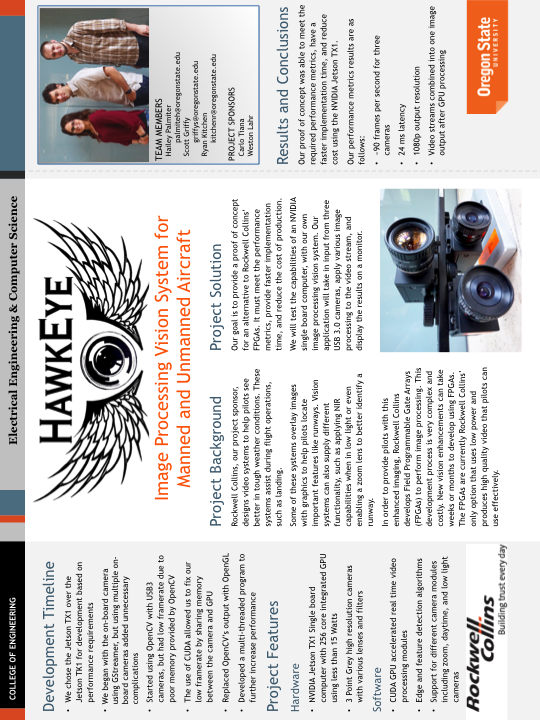
\includegraphics[width=\textwidth,height=\textheight,keepaspectratio]{images/HawkEye_Poster.png}  
	\end{figure}

\section{Project Documentation}
	\subsection{Project Overview}
Our project is a proof of concept to determine the usability of the NVIDIA Jetson TX1 for aerospace computer vision applications.  It demonstrates this capability by processing multiple video streams with multiple image filters at high frame rates and low latency. This program is designed to run without needing any interaction from the user, however we have included the ability to switch between different video processing modes in order to demonstrate the various filters and camera views.
The HawkEye Vision System captures video from cameras, processes it using various filter algorithms, and displays it on the screen. It utilizes both the CPU and GPU simultaneously to create a very high throughput, low latency video feed. The CPU portion of the program is responsible for capturing video from the camera using Point Grey?s Flycapture API, and managing the parameters of the GPU programs (which are called kernels). The CPU program also manages user input and sets up the OpenGL output system. 

\begin{figure}[H] 
	\centering
	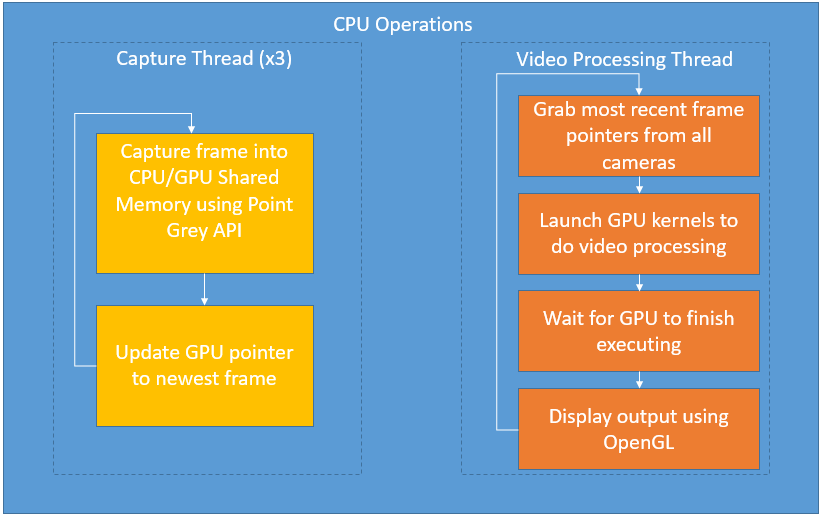
\includegraphics[width=0.6\textwidth,natwidth=610,natheight=642]{images/CPU.png} 
	\caption{CPU Operation - showing the functions of the different CPU threads}  
	\end{figure}
	
The GPU does all the heavy lifting in this program. It performs multiple video processing operations simultaneously. The GPU program is divided into several streams, each of which operates independently of the others, much like the multiple threads on a CPU. The Jetson allows multiple GPU kernels to run at the same time, as long as they are in different streams.
In the following diagram, each box represents a different GPU Kernel (with the exception of the bottom right box which is actually the same as the three bottom left kernels, just abbreviated to save space). These kernels are executed in order by their corresponding CUDA streams, which is essential. 
	
\begin{figure}[H] 
	\centering
	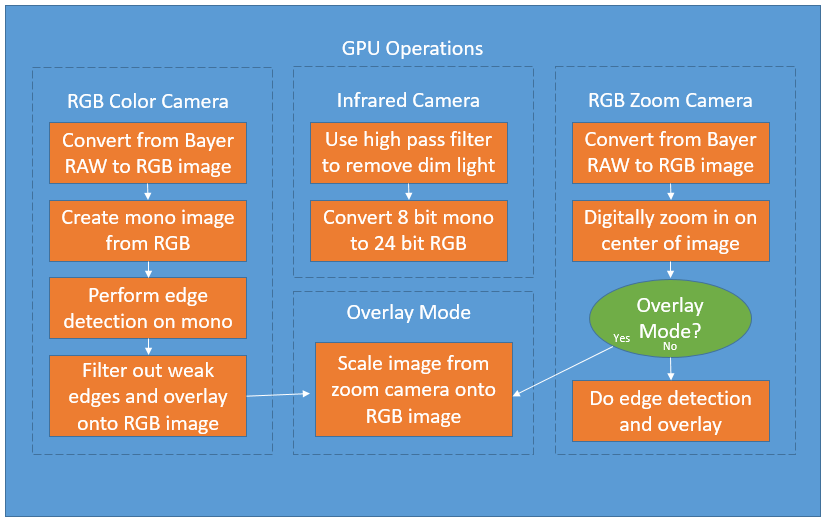
\includegraphics[width=0.6\textwidth,natwidth=610,natheight=642]{images/GPU.png}
	\caption{GPU Operation - showing the functions of the different CUDA streams}  
	\end{figure}
	
\subsection{Installation and Execution}
This software is designed to be a proof of concept that demonstrates the computing power of the NVIDIA Jetson TX1. It is not meant to be installed on other hardware, as it requires the use of the GPU present in the Jetson, and is specifically optimized to use the Jetson?s CPU/GPU shared memory that is not present on other devices. There are a number of example programs created using various filters and elements of the HawkEye system. They are run simply by executing them on the console.
\par
This software is designed specifically for the NVIDIA Jetson TX1 and for use with Point Grey USB 3.0 Cameras. It can be recompiled for other systems with CUDA-enabled GPUs however this has not been tested.

\subsection {Example Controls}
The example program we used at Expo has several controls.\\

Camera Views:
\begin{description}[leftmargin=2cm,labelindent=2cm]
	\item[{[1]}] RGB Camera
	\item[{[2]}] NIR Camera
	\item[{[3]}] Zoom Camera\\
\end{description}

Filters:
\begin{itemize}[leftmargin=2cm,labelindent=2cm]

\item RGB and Zoom Camera Views:
\begin{description}[leftmargin=2cm,labelindent=2cm]
	\item[{[G]}] Enable edge detection
	\item[{[F]}] Disable edge detection
	\item[{[H]}] Decrease edge detection threshold (more edges)
	\item[{[J]}] Increase edge detection threshold
	\item[{[\{]}] Zoom out
	\item[{[\}]}] Zoom in
\end{description}

\item RGB Only:
\begin{description}[leftmargin=2cm,labelindent=2cm]
	\item[{[Z]}] Enable zoom overlay
	\item[{[X]}]  Disable zoon overlay
\end{description}

\item IR Only:
\begin{description}[leftmargin=2cm,labelindent=2cm]
	\item[{[A]}] Decrease IR Threshold (brighter image)
	\item[{[S]}]  Increase IR Threshold (see only bright lights)\\
\end{description}

\end{itemize}

Quit Programs:
\begin{description}[leftmargin=2cm,labelindent=2cm]
	\item[{[Q]}]  Quit
\end{description}


	
\newpage
\section{Discovery of New Technologies}
	The primary resource used for this project was the CUDA 7.0 User manual, found on NVIDIA's website. This manual contains a best practices guide which explains how to use various optimizations and produce code that best takes advantage of the GPU hardware. 
\par
The edge detection algorithm we used is an adaptation of the LSD Line Segment Detector, which was originally developed as a graduate research project. The original research article can be found at http://www.ipol.im/pub/art/2012/gjmr-lsd/.
\par
Lastly we made use of various documentation from Point Grey, which described how to set up the cameras, alter various settings, and determine the appropriate Bayer conversion mode (there are multiple different input types). Their website is www.ptgrey.com.\\


\newpage	
\section{Personal Experiences}
	\subsection{Hailey Palmiter}
		\subsubsection{What technical information did you learn?}
I began this project with no real background in hardware and no background in vision systems to include graphics libraries. Therefore the entire technical side of our project was a learning experience for me. It started with the use of the Jetson TK1 and TX1 development environment that used Ubuntu. I have interacted with the Linux operating system in the Operating Systems classes. The PointGray camera had their own drivers we had to install and work with. PointGrey also included its own graphical user interface called FlyCapture that we had to manipulate. Thus we needed to understand what was happening within those packages and interface in order to have it do what we needed it to. 
\par
The language I got the most exposure with was OpenGL we had to interact with several of its libraries and its toolkit called GLUT. I also learned about CUDA and using CUDA kernels to handle filter operations on our captured image buffers. I learned how an image is captured from the camera and stored into a buffer, which we created into a shared buffer between the GPU and CPU. I also learned how to use parallel processing with image buffers to increase latency and frame rate speeds. 
\par
During the creating of the runway I was also able to work with a micro controller in order to program our LED strip lights to produce a runway like approach lighting system.\\

\subsubsection{What non-technical information did you learn?}
A few non-technical things that I learned involved creating latex documents, FAA runway standards, and creating formal documentation on our project. Using latex and the IEEEtran formatting style we were able to create very professional looking documents. There was a steep learning curve for latex, but once I had figured it out it made all of our documentation very simple to create. Even though I had learned about requirements documents, design documents, and technical reviews in the Software Engineering classes, it was a whole new learning experience creating them for a real industry like project. 
\par
Another non-technical experience was learning how interact and deal with a client. During the planning process of our project we had to have a lot more involvement with our client to make sure we were establishing all of the requirements they had for us and were also creating the project they had in mind. Later in development I had to keep them updated with our progress, set up meeting, create an outline for the meetings along with producing meeting minutes after it had concluded. Throughout the entire project we needed to assure that they were informed and happy with what we were doing for them, while also follow the requirements document we had established.\\

\subsubsection{What have you learned about project work?}%Finish
I have learned that there are a lot of moving parts to a project and that it is much

\subsubsection{What have you learned about project management?}
I have learned that project management runs much smoother once you are able to find out how other people work. Knowing your team, their strengths and weaknesses, availability, and how they work best is a piece of how to lead people well. I learned how to set each of my team members up for success by assigning tasks appropriately based on what they enjoyed, what they were good at, and the time they had to work on a specific task. 
\par
I also learned that staying organized and setting deadlines/goals for things help us all to stay focused and to complete the things we needed to on time.\\

\subsubsection{What have you learned about working in teams?}
I have learned that working in a team doesn't matter if you are all the best of friends, but what matters is being able to leave it all at the door to create a professional work environment where all entities are comfortable and feel as being an important piece of the project. I was lucky that our team all got a long well and worked really well together, but I believe it also taught me what a good team dynamic should look and feel like. Each of us had a strength to bring to the project, which created a very strong team dynamic. I also learned about compromising with others on ideas as well as being able to help support team members with tasks when needed.\\ 

\subsubsection{If you could do it all over, what would you do differently?}

	\subsection{Scott Griffy}
		\subsubsection{What technical information did you learn?}
I learned a lot about the hardware of single board computers. I often work with graphics on desktops, but you don't have to dive into the hardware when you're working on a desktop, all the functionality is given to you through library calls and APIs. On the Jetson we literally had to recompile the kernel at times to get more functionality out of the board. I've never had to recompile a kernel to complete a project and knowing how to do so improved the technical tools I have at my disposal for computer projects.
\par
I also learned a lot on the software side of graphics processing. I learned about CUDA and the cuda libraries, especially how to maximize the performance when I'm working with graphics libraries. When I'm working on higher-level projects, most of the performance enhancements I make are in the algorithm, but when you're working with low level hardware, the difference is in the implementation. Memory copies are the enemy in latency for graphics systems and after we minimized those with custom buffers for the camera capture and GPU textures, we got the best latency. I also learned more about how camera capture APIs work and how to access the physical registers on a camera.
\par
I feel that I learned more technical stuff that will help me in future projects if needed, but I can't specifically recall it here.
\subsubsection{What non-technical information did you learn?}
\par
I think the biggest takeaway that I got out of this project was working with a team in a long term project like this. I've worked in groups on smaller projects before but never for a whole year. In some ways working with a group for a longer amount of time is easier and in some ways it's harder. In a short project, the difficulty is learning how to work with the group in the short amount of time. When you open it up to a larger project, you realize that group projects 
\par
I also learned about how to explain technical things to a non-techincal audience. This was important for some of the documents we wrote as well as at expo. Often, when I'm working on a project, I get caught up in the code and never boil it down so that I can explain it to people. This might be the most important part of any technical work, explaining it to other people so it can be used and improved upon.
\subsubsection{What have you learned about project work?}
\par
When you're working on a project, you need to make sure that you're on task and that the task you're doing is important. This is the most important part of project work and a lot of the effort in a project goes towards defining these tasks. If your project is well thought-out and you're on task, the project will get completed and be successful and if you've met and defined good requirements, then all you need to do when you're working on your own is stay on task. This might seem simple, but it's really easy to get off task and try to feature creep on your own, or end a meeting early deciding that you'll figure out the rest of the tasks on your own. These are both examples of bad project work and should be avoided.
\subsubsection{What have you learned about project management?}
\par
Setting up meetings and assigning work isn't always easy. Sometimes the correct path isn't clear, but you still have to make a decision. Sometimes you don't have time to weigh all the options and simply need to choose a route that might not be optimal. Management is about a lot of small things and corner cases. There's never a correct answer and you never make the best decisions. The important part is simply making decisions and not being entirely wrong. Because making an okay decision is a lot better than making no decision at all.
\subsubsection{What have you learned about working in teams?}
\par
When you're working in teams with people you have to worry about workloads. You don't want one person to do all the work while the others have too much free time. That's why the work needs to be split up.
\subsubsection{If you could do it all over, what would you do differently?}
\par
If I could do it all over again, I wouldn't change much. We really did the best we could at each stage of the project. Maybe I would've been more involved with the image processing algorithms, because I fell behind a bit and was playing catch up learning the vision processing algorithms at the end of the term.

	\subsection{Ryan Kitchen}
		\subsubsection{What technical information did you learn?}
\subsubsection{What non-technical information did you learn?}
\subsubsection{What have you learned about project work?}
\subsubsection{What have you learned about project management?}
\subsubsection{What have you learned about working in teams?}
\subsubsection{If you could do it all over, what would you do differently?}

\begin{appendices}	

\newpage
\section{Essential Code Listings}
	%\lstinputlisting{code/CODE_FOR_FINAL_DOC}
Unless otherwise specified, all code is in /HawkEyed\_Video/HawkEye\_2.0.\\
\par
The following code is the buffered camera system that is used in our final product.
The "Frame" type is a class we designed that maintains the data until it is done being used
and then releases it to be captured into again.\\
\lstinputlisting{code/camera_2.0.cpp}
\par
This code is the edge detection algorithm used in the demo. It uses a pixel and 3 of its neighbors
to determine the direction and magnitude of a change in brightness. This example shows how to develop a
CUDA kernel and some of the optimizations we used in order to reduce latency.\\
\lstinputlisting{code/edge_overlay.cu}
\par
This code is the main program for our demonstration application, which was used for the benchmarking
and at expo. It shows how different kernels can be strung together via streams, and the operations changed during
program execution.\\
\lstinputlisting{code/glut_output.cpp}
\par
This code is our pipeline system, which was developed and used to achieve even lower latency  for our software, but 
was not included in the final version because of stability issues, but would be the preferred method for future development.
It demonstrates a more effective way to process multiple frames at the same time, and optimizes to only grab the most
recent frames instead of processing all frames in order. It allows the programmer to avoid directly having to implement 
multithreaded, multi-stream processing, and instead focus on just the algorithm development.\\
\lstinputlisting{code/pipeline.h}
	
\newpage	
\section{Hardware and Output Image Examples}
	\subsection{Hardware}
   This section includes a list of all the hardware we have been (very generously) lent and have been working with for the duration of this project. The following list and images should be able to supply a better understanding and familiarization of the project.\\
	\\Cameras (figure 1):  
    		\begin{itemize}
		\item GS3-U3-41C6NIR-C (PointGrey/GrassHopper)
		\item GS3-U3-41C6C-C
		\item GS3-U3-23S6C-C\\
		\end{itemize}
	Lenses (figure 1): 
		\begin{itemize}
		\item EVS-3000 (figure 6)
		\item 2 x LS-TP-08 (Standard) (figure 7)\\
		\end{itemize}					
	Single Board Computers: 
		\begin{itemize}
		\item Jetson TK1 (figure 2) 
		\item Jetson TX1 developer kit with on-board camera (figure 3 and 4)\\
		\end{itemize}		
	Extras: 
		\begin{itemize}
		\item NIR Pass filter - blocks visible light while allowing NIR light through
		\item 2-port USB 3.0 supersede PCIe Card (figure 5)
		\item Camera mount
		\item 3 x USB 3.0 cables
		\item 1080p monitor (TV)\\
		\end{itemize}
		
\begin{figure}[!ht]
	  \centering
		    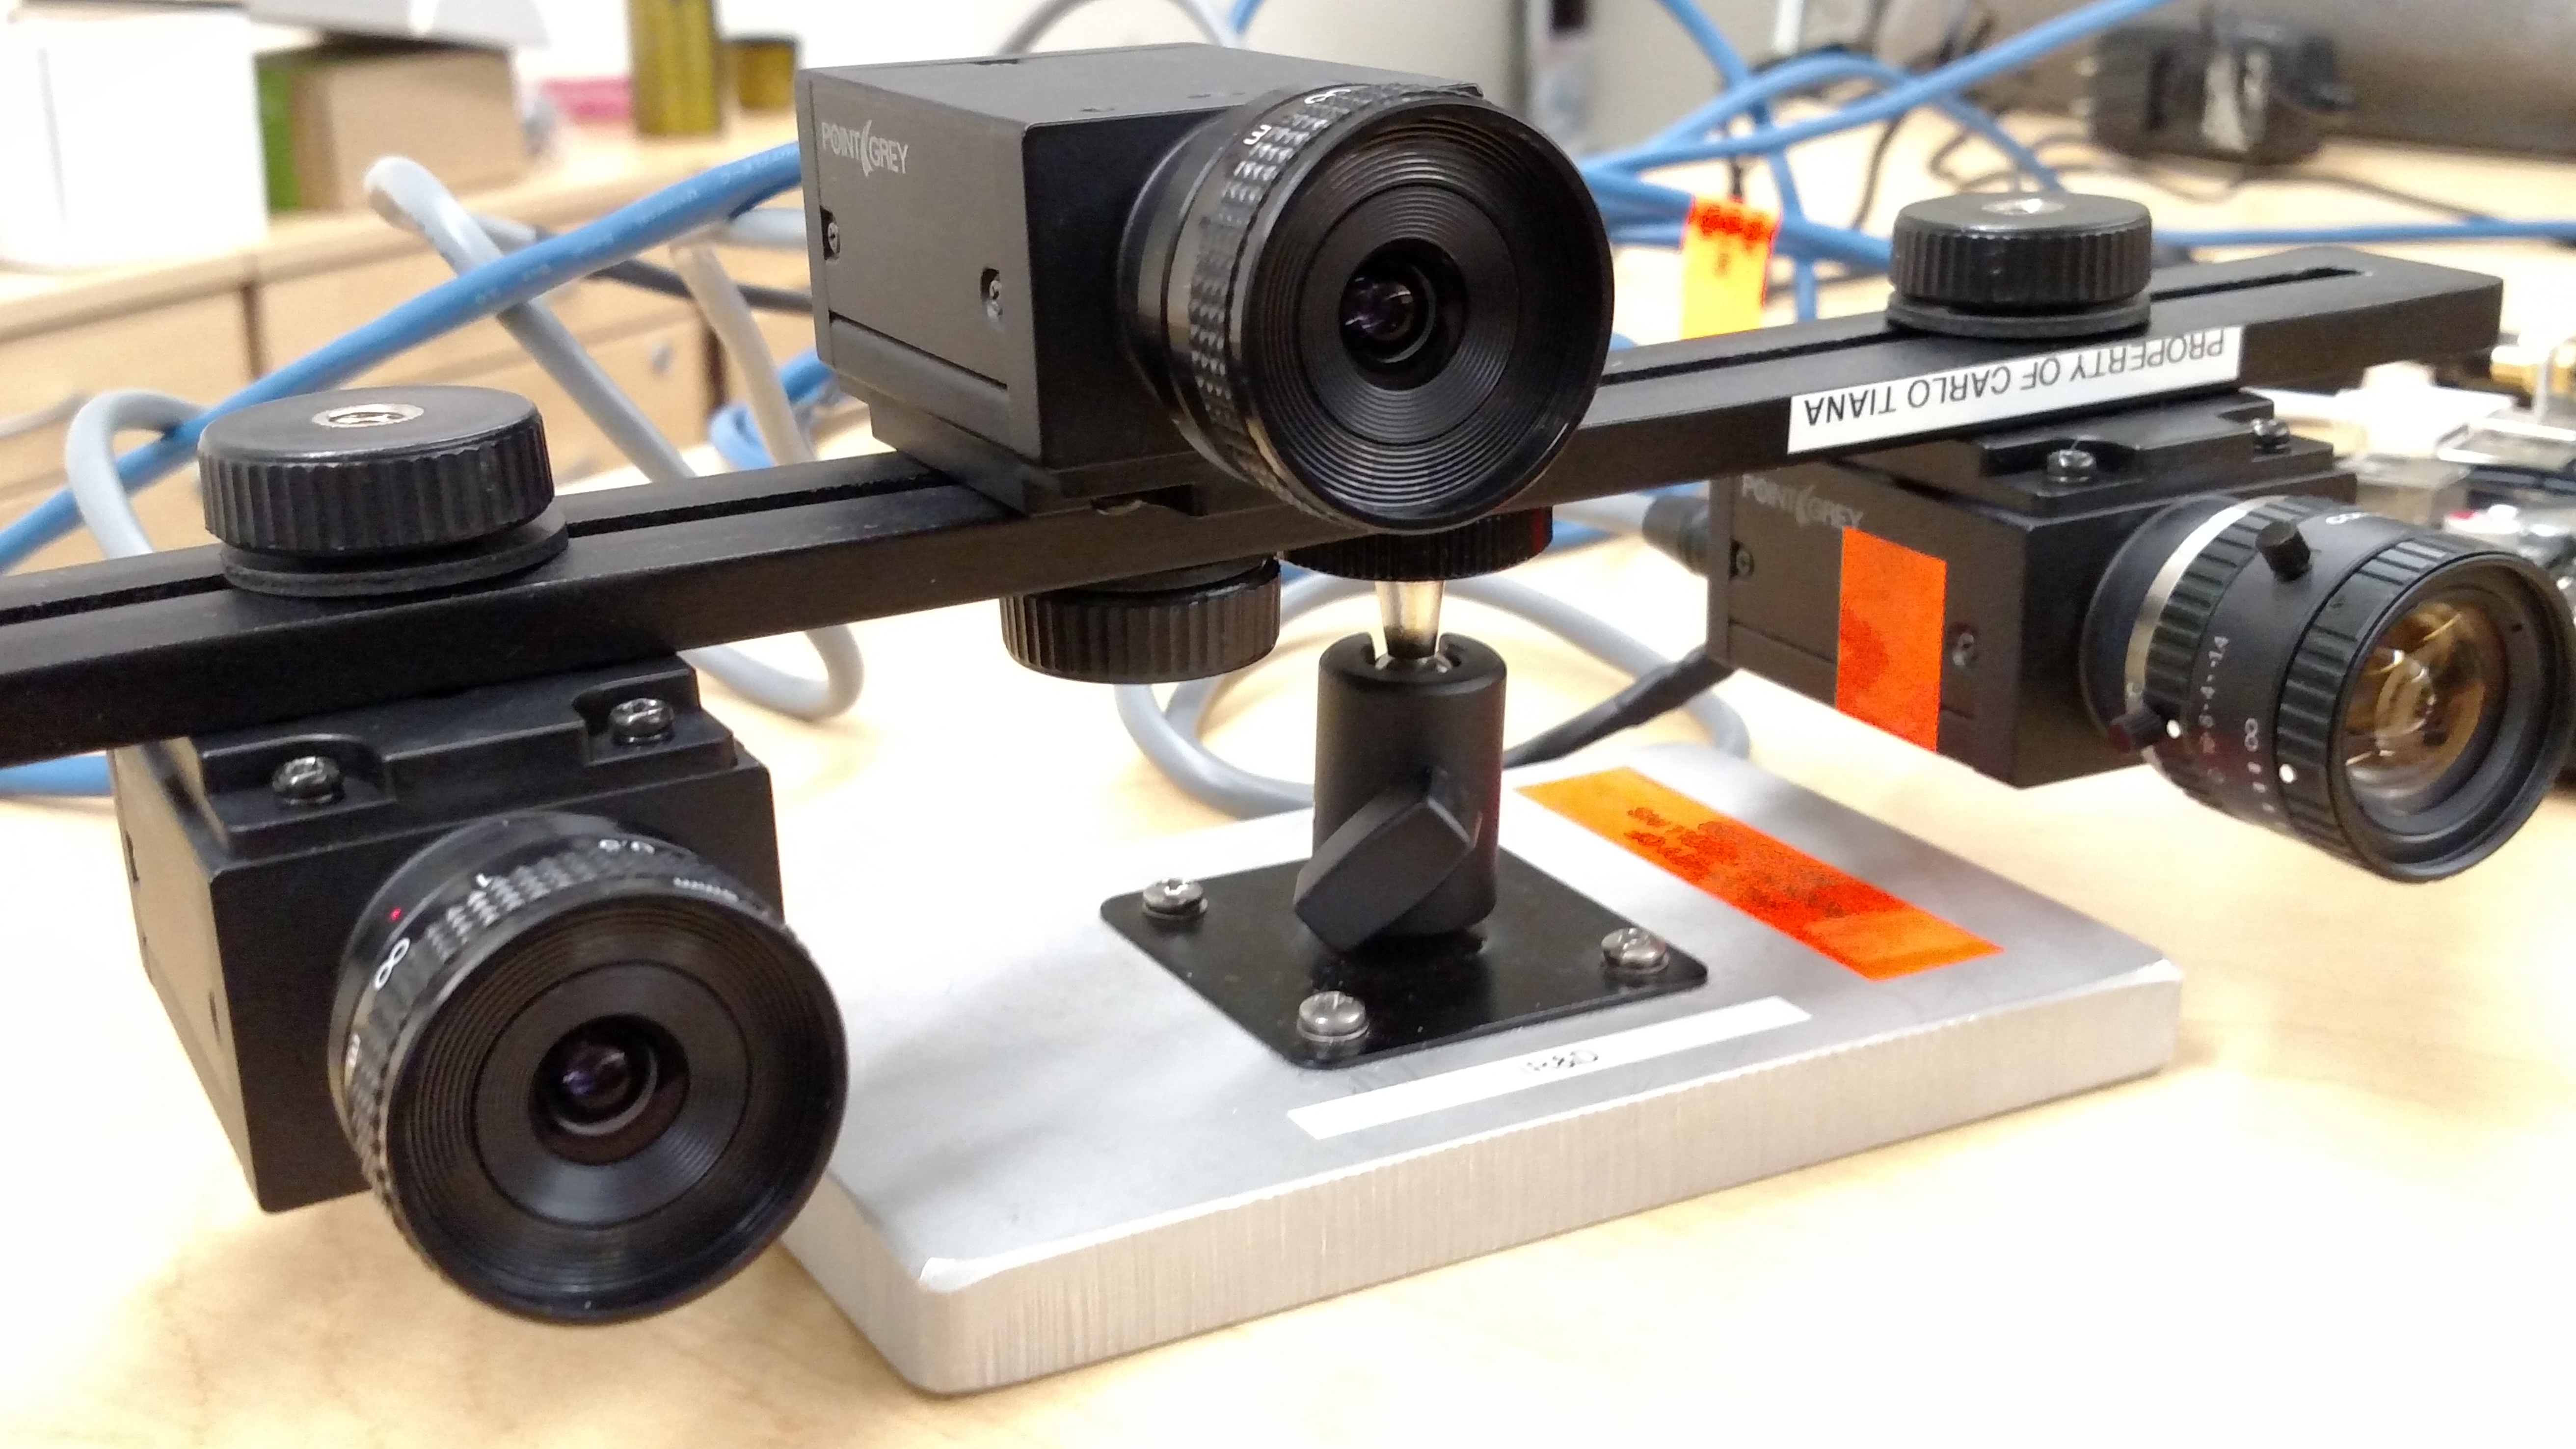
\includegraphics[width=0.6\textwidth,natwidth=610,natheight=642]{images/cameras.jpg}
		    \caption{The 3 PointGrey cameras provided by Rockwell Collins on a mount}
				\end{figure} 
 \begin{figure}[!ht]
	  \centering
		    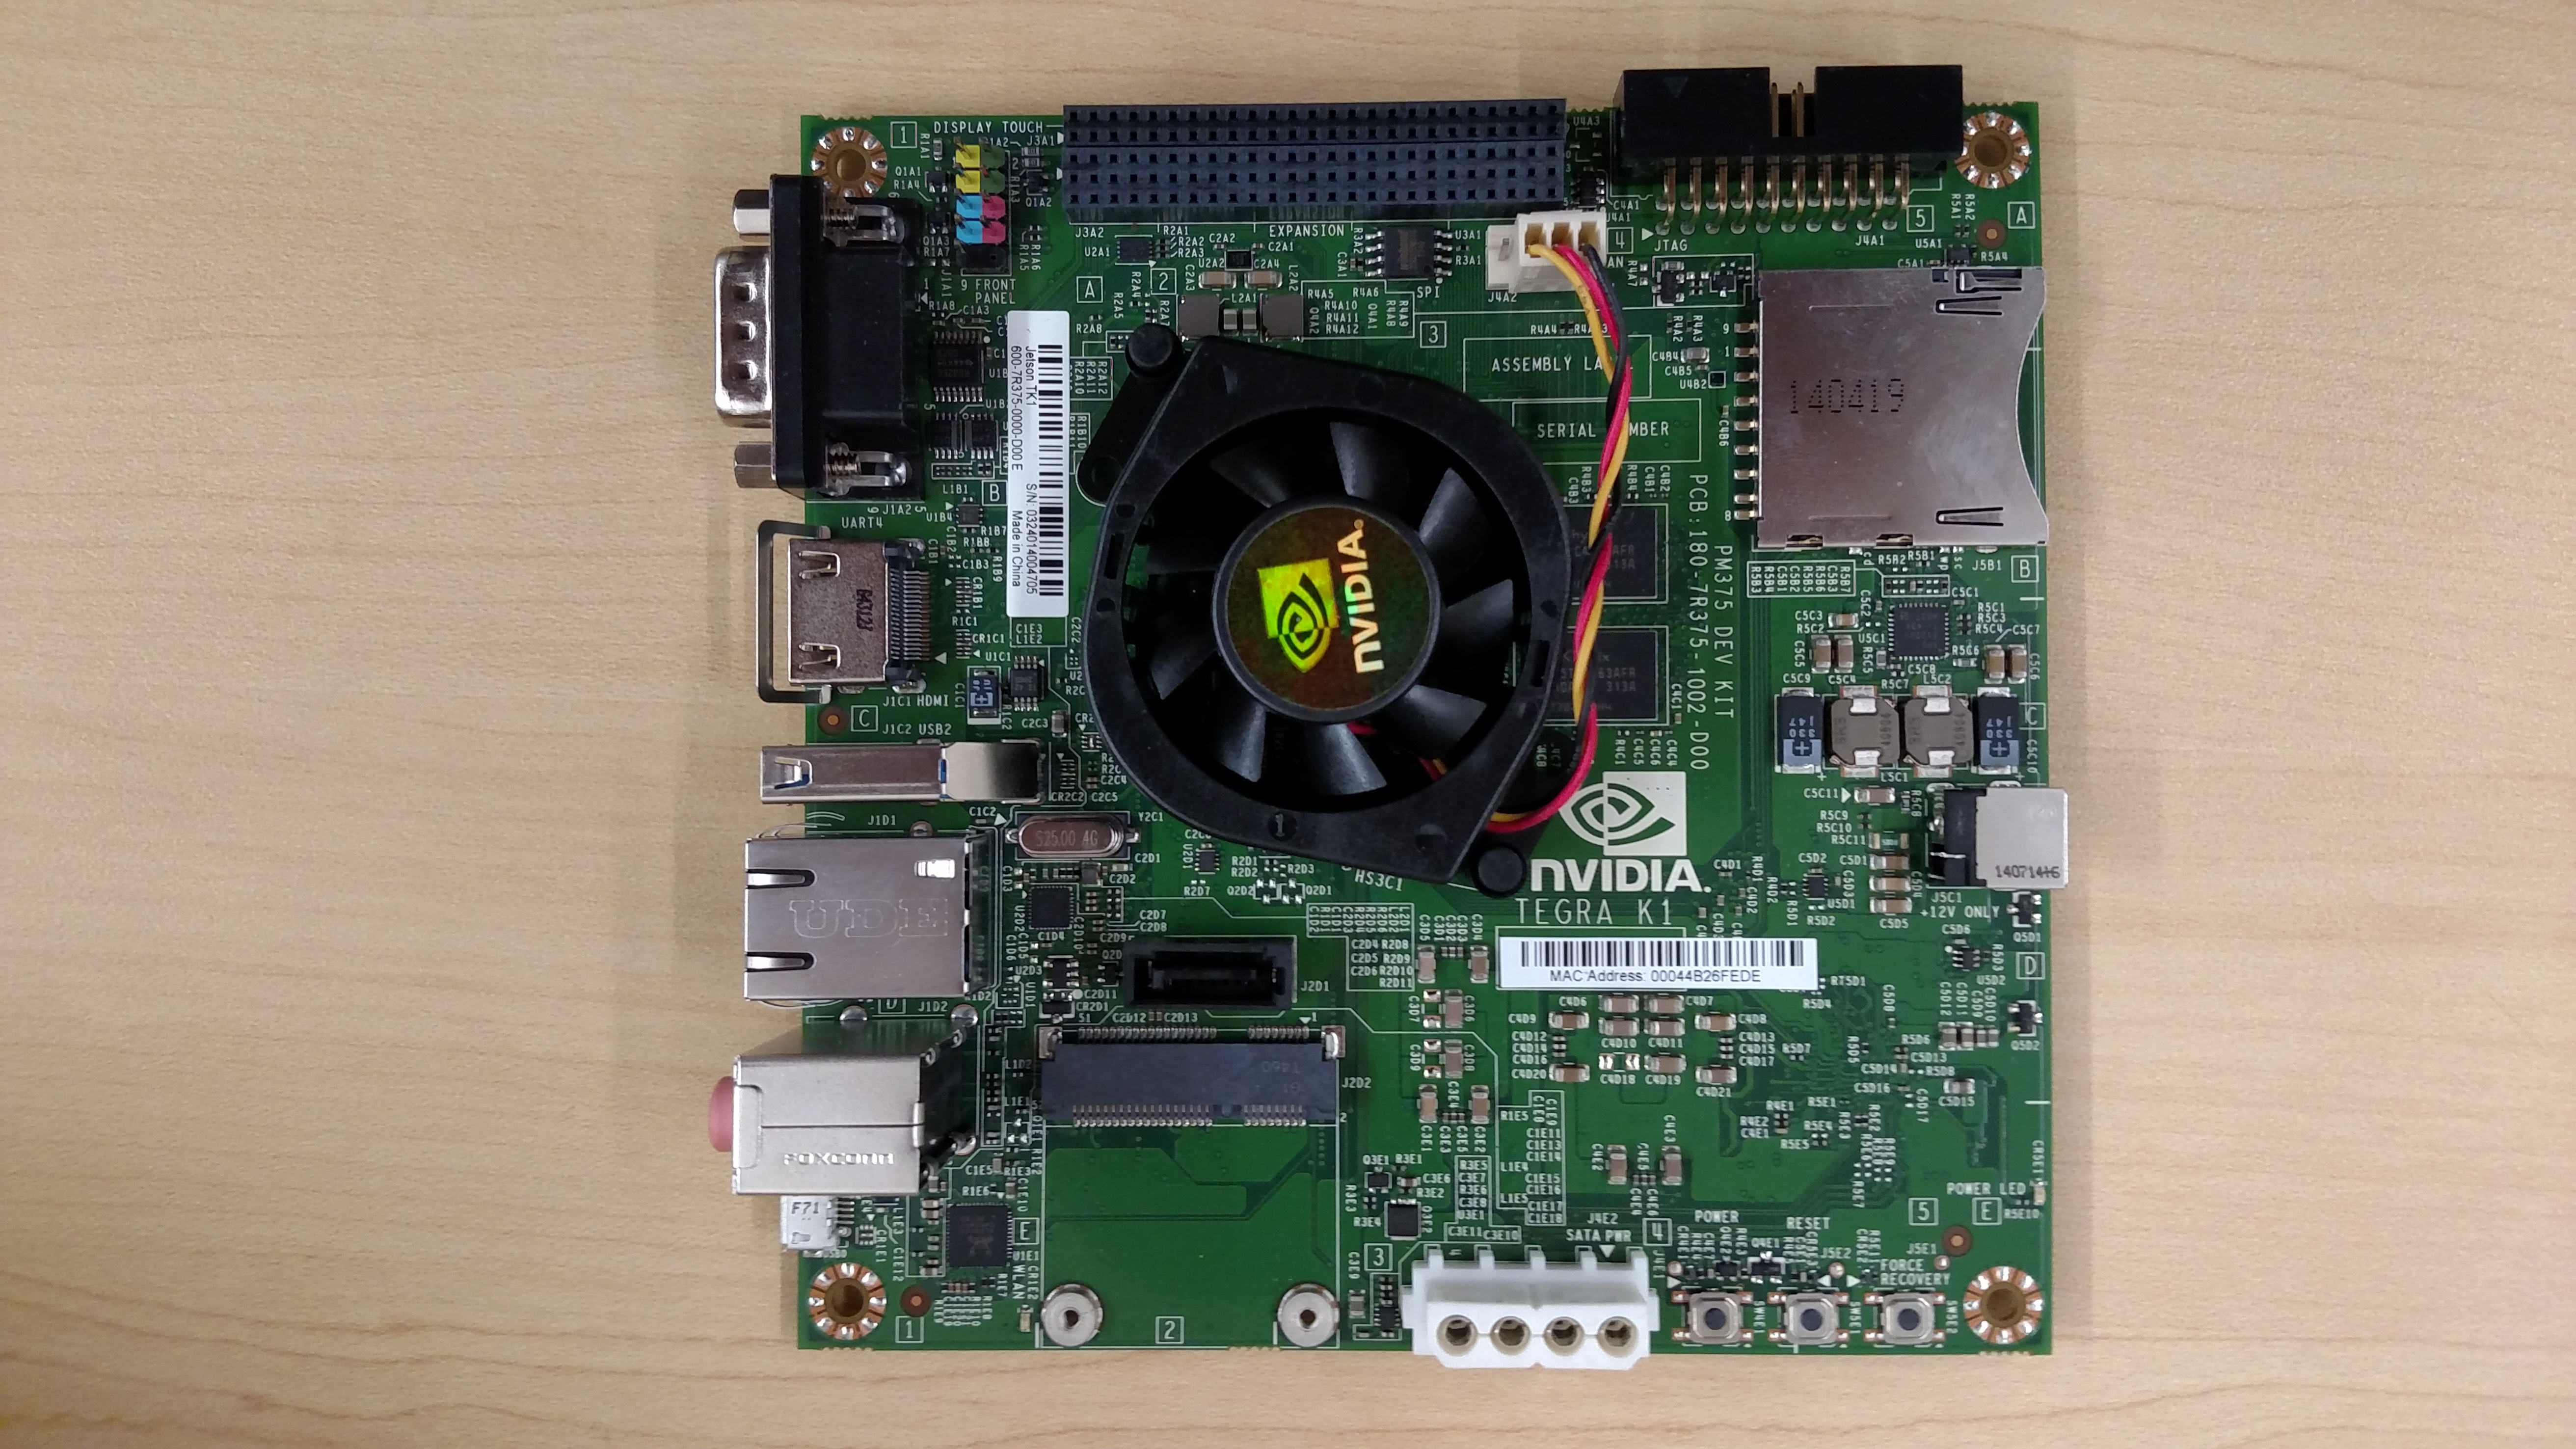
\includegraphics[width=0.6\textwidth,natwidth=610,natheight=642]{images/JetsonTK1.jpg}
		      \caption{The Jetson TK1}
				\end{figure}
\begin{figure}[!ht]
	  \centering
		    \includegraphics[width=0.6\textwidth,natwidth=610,natheight=642]{images/JetsonTX1.jpg}
		      \caption{The Jetson TX1}
				\end{figure}
\begin{figure}[!ht]
	  \centering
		    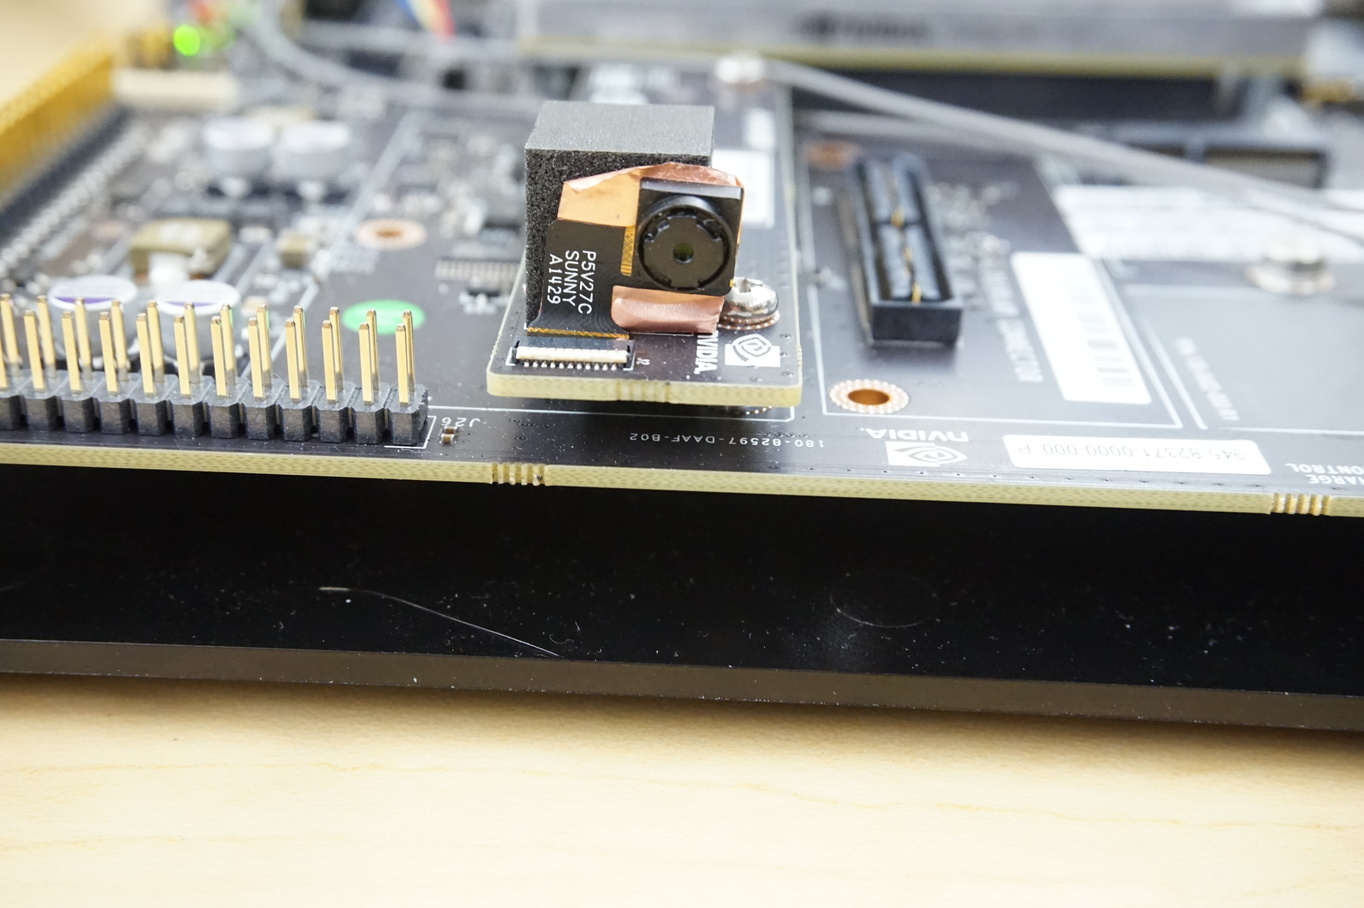
\includegraphics[width=0.6\textwidth,natwidth=610,natheight=642]{images/onboardCamera.JPG}
		     \caption{The on-board camera for the TX1}
				\end{figure}

\begin{figure}[!ht]
	  \centering
		    \includegraphics[width=0.6\textwidth,natwidth=610,natheight=642]{images/PCIe.jpg}
		      \caption{2-port USB 3.0 supersede PCIe Card}
				\end{figure}

\newpage
\subsection{Output Display Images}

Below are a few different images we were able to obtain with the use of our hardware and a few simple filters. Figure 6 and 7 are showing the original unprocessed output stream. Figure 6 is using the EVS-3000 lens and figure 7 is using the standard LS-TP-08 lens.\\

   \begin{figure}[!ht]
	  \centering
		    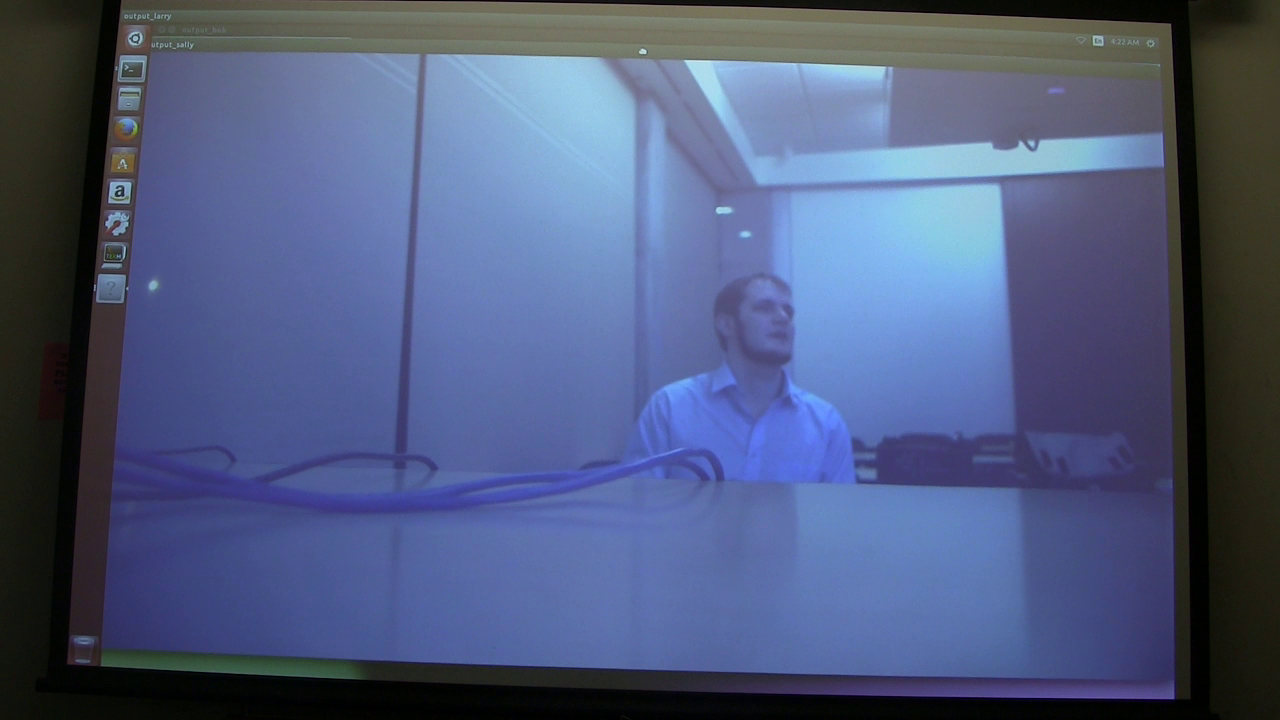
\includegraphics[width=0.6\textwidth]{images/normal_image.png}
		      \caption{Video output from the TX1 using a PointGrey camera with an EVS-3000 lens attached}
				\end{figure}
				
\begin{figure}[!ht]
	  \centering
		    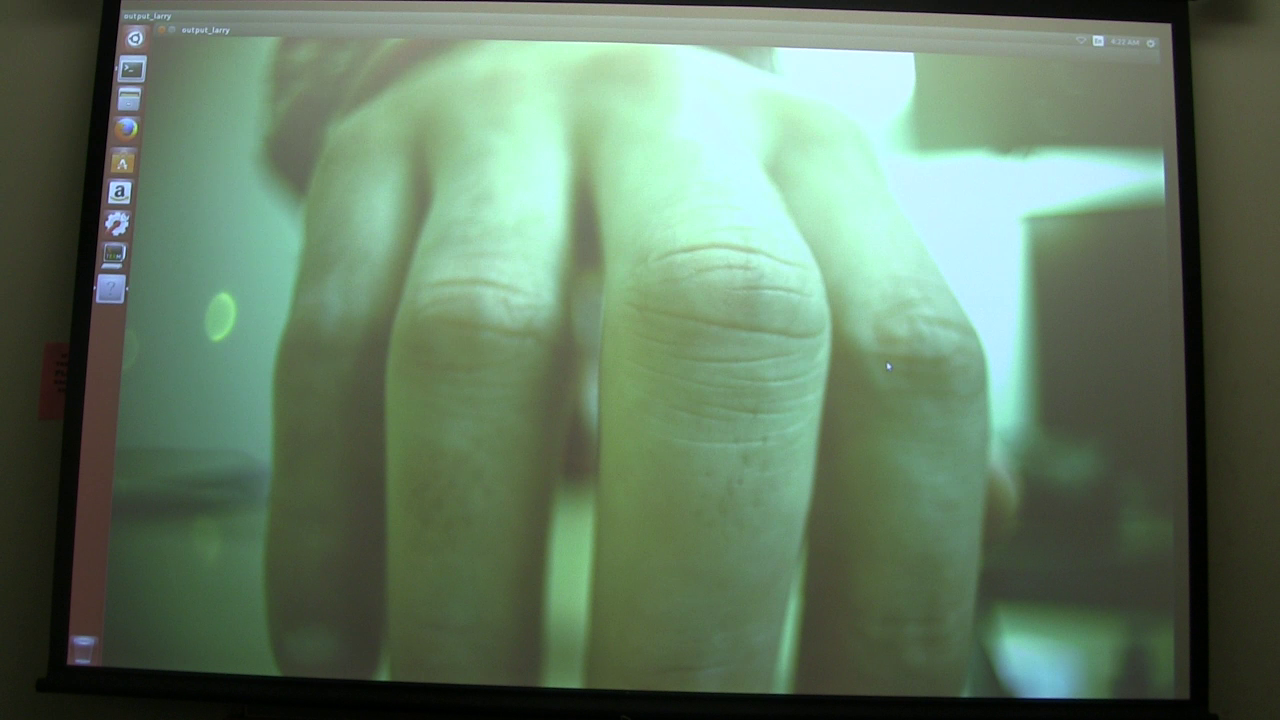
\includegraphics[width=0.6\textwidth]{images/green_image.png}
		      \caption{Video output from the TX1 using a PointGrey camera with a LS-TP-08 lens attached}
				\end{figure}

\begin{figure}[!ht]
	  \centering
		    \includegraphics[width=0.6\textwidth]{images/line_detection.png}
		      \caption{Video output from the TX1 using a built-in OpenCV line detection filter}
				\end{figure}
 				
\begin{figure}[!ht]
	  \centering
		    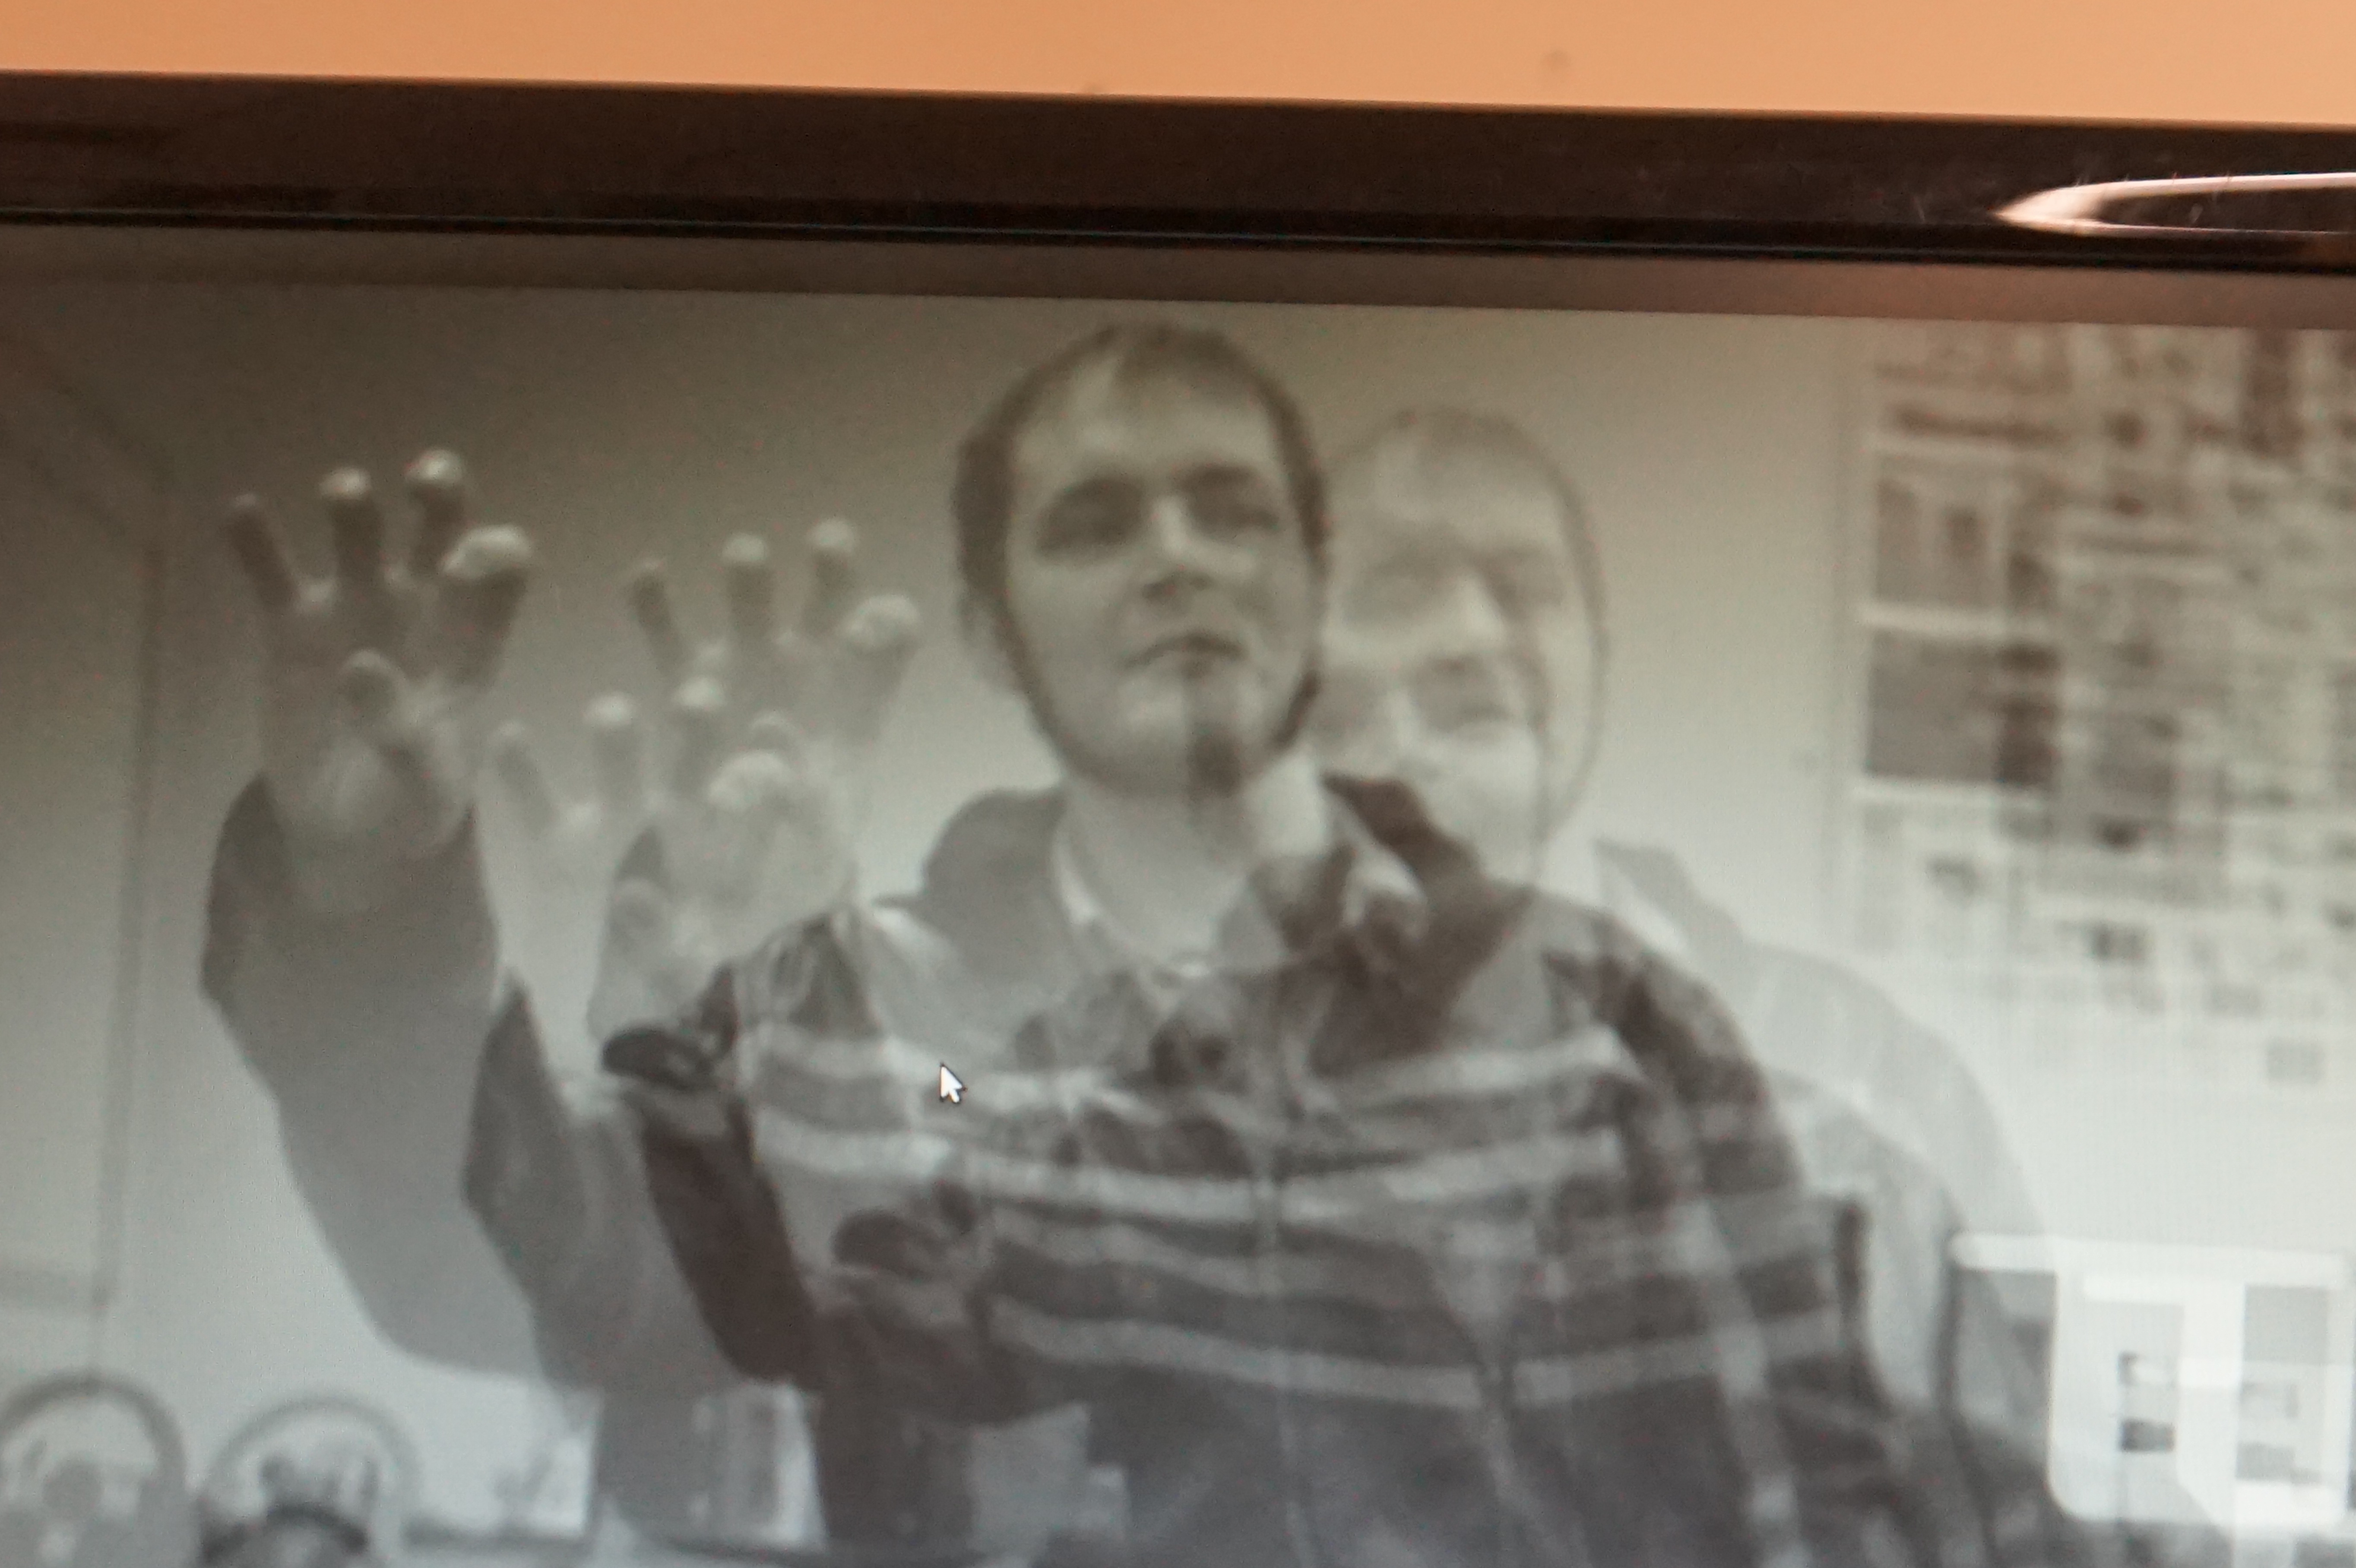
\includegraphics[width=0.6\textwidth]{images/3_normal.png}
		      \caption{Video output from the TX1 overlaying three USB 3.0 video streams}
				\end{figure}
			
\begin{figure}[!ht]
\centering
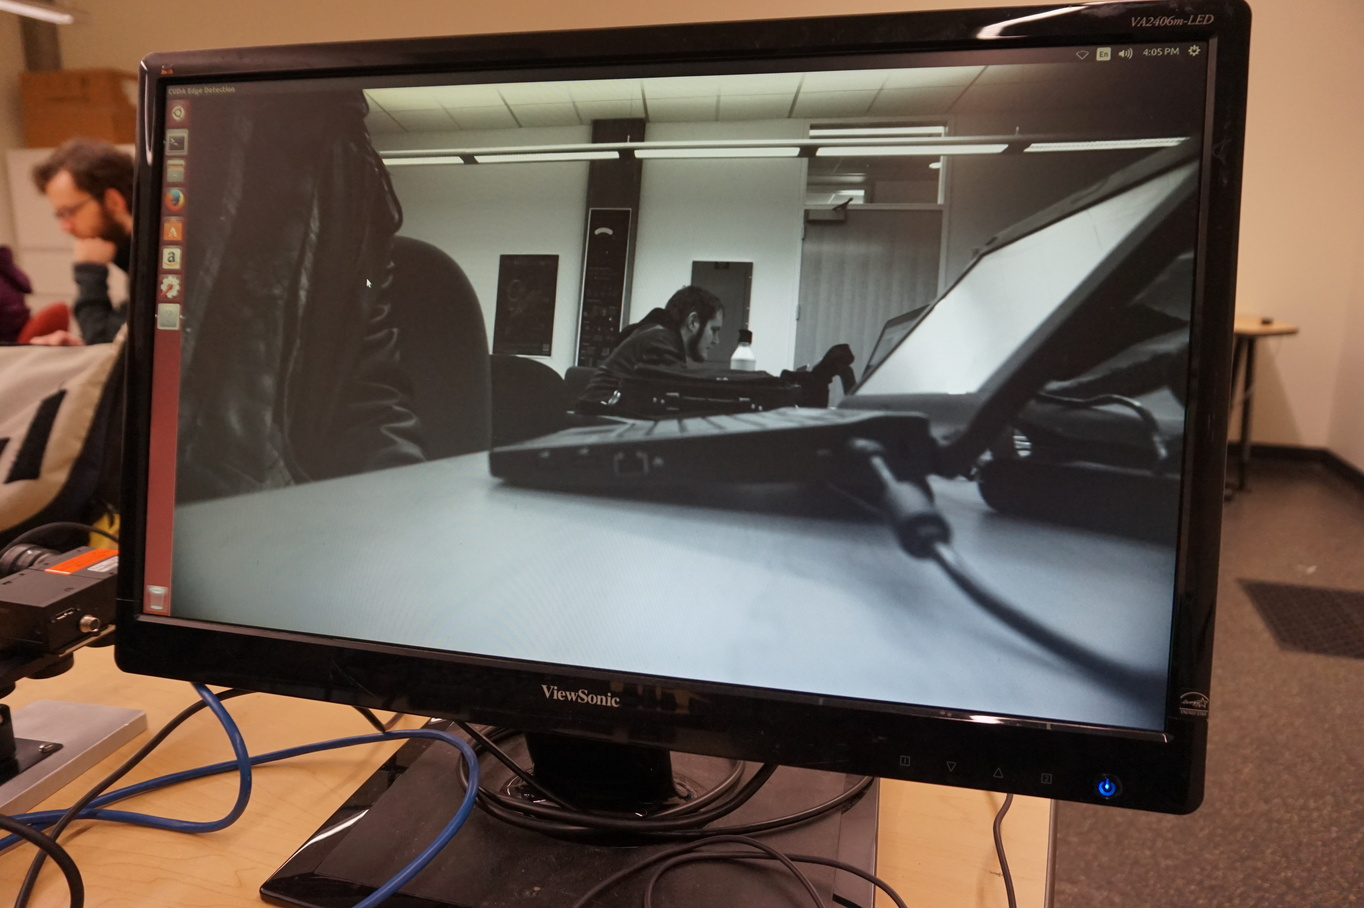
\includegraphics[width=0.6\textwidth]{images/exampleOutputNormalBeta.jpg}
\caption{Video output from the TX1 running at ~85 fps}
\end{figure}

\end{appendices}
   
\end{document}
